\section{平面问题的极坐标解答}
\subsection{极坐标中的平衡微分方程}
\begin{figure}[!h]
\centering
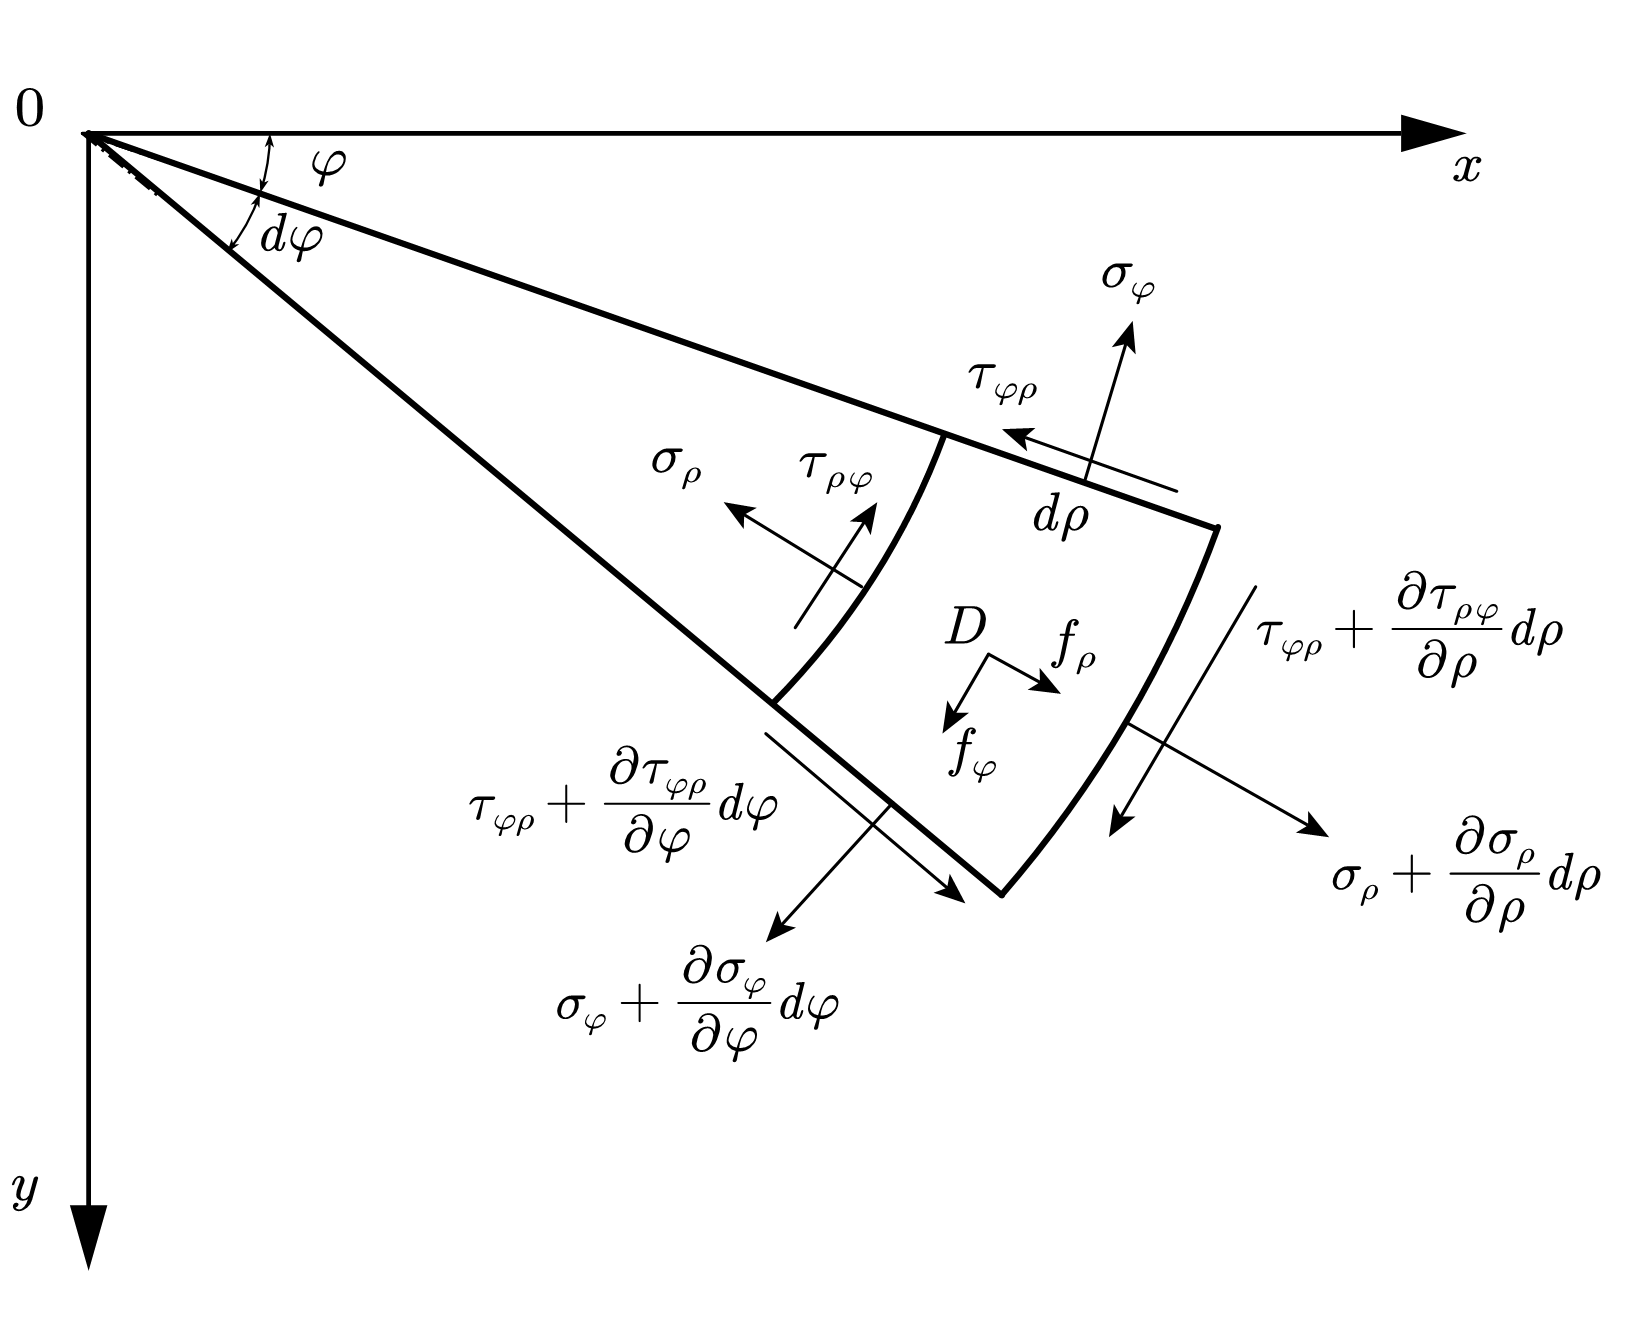
\includegraphics[scale=0.5]{figure/4-1.png}
\caption{}
\end{figure}
\subsubsection{极坐标中的平衡微分方程}
\begin{equation}
\begin{cases}
\frac{\partial \sigma _{\rho}}{\partial \rho}+\frac{1}{\rho}\frac{\partial \tau _{\rho \varphi}}{\partial \varphi}+\frac{\sigma _{\rho}-\sigma _{\varphi}}{\rho}+f_{\rho}=0\\
\frac{1}{\rho}\frac{\partial \sigma _{\varphi}}{\partial \varphi}+\frac{\partial \tau _{\rho \varphi}}{\partial \rho}+\frac{2\tau _{\rho \varphi}}{\rho}+f_{\varphi}=0\\
\end{cases}
\end{equation}

\subsection{极坐标中的几何方程和物理方程}
\subsubsection{极坐标中的几何方程}
\begin{equation}
\begin{cases}
\varepsilon _{\rho}=\frac{\partial u_{\rho}}{\partial \rho}\\
\varepsilon _{\varphi}=\frac{u_{\rho}}{\rho}+\frac{1}{\rho}\frac{\partial u_{\rho}}{\partial \varphi}\\
\gamma _{\rho \varphi}=\frac{1}{\rho}\frac{\partial u_{\rho}}{\partial \varphi}+\frac{\partial u_{\rho}}{\partial \rho}-\frac{u_{\varphi}}{\rho}\\
\end{cases}
\end{equation}
\subsubsection{极坐标中的物理方程}
\begin{equation}
\begin{cases}
\varepsilon _{\rho}=\frac{1}{E}\left( \sigma _{\rho}-\mu \sigma _{\varphi} \right)\\
\varepsilon _{\varphi}=\frac{1}{E}\left( \sigma _{\varphi}-\mu \sigma _{\rho} \right)\\
\gamma _{\rho \varphi}=\frac{1}{G}\tau _{\rho \varphi}=\frac{2\left( 1+\mu \right)}{E}\tau _{\rho \varphi}\\
\end{cases}
\end{equation}
平面应变的情况下,需将上式中的$E$换为$\frac{E}{1-\mu ^2}$,$\mu$换为$\frac{\mu}{1-\mu}$。

\subsection{坐标变换}
\subsubsection{位移分量的坐标变换}
\begin{figure}[!h]
\centering
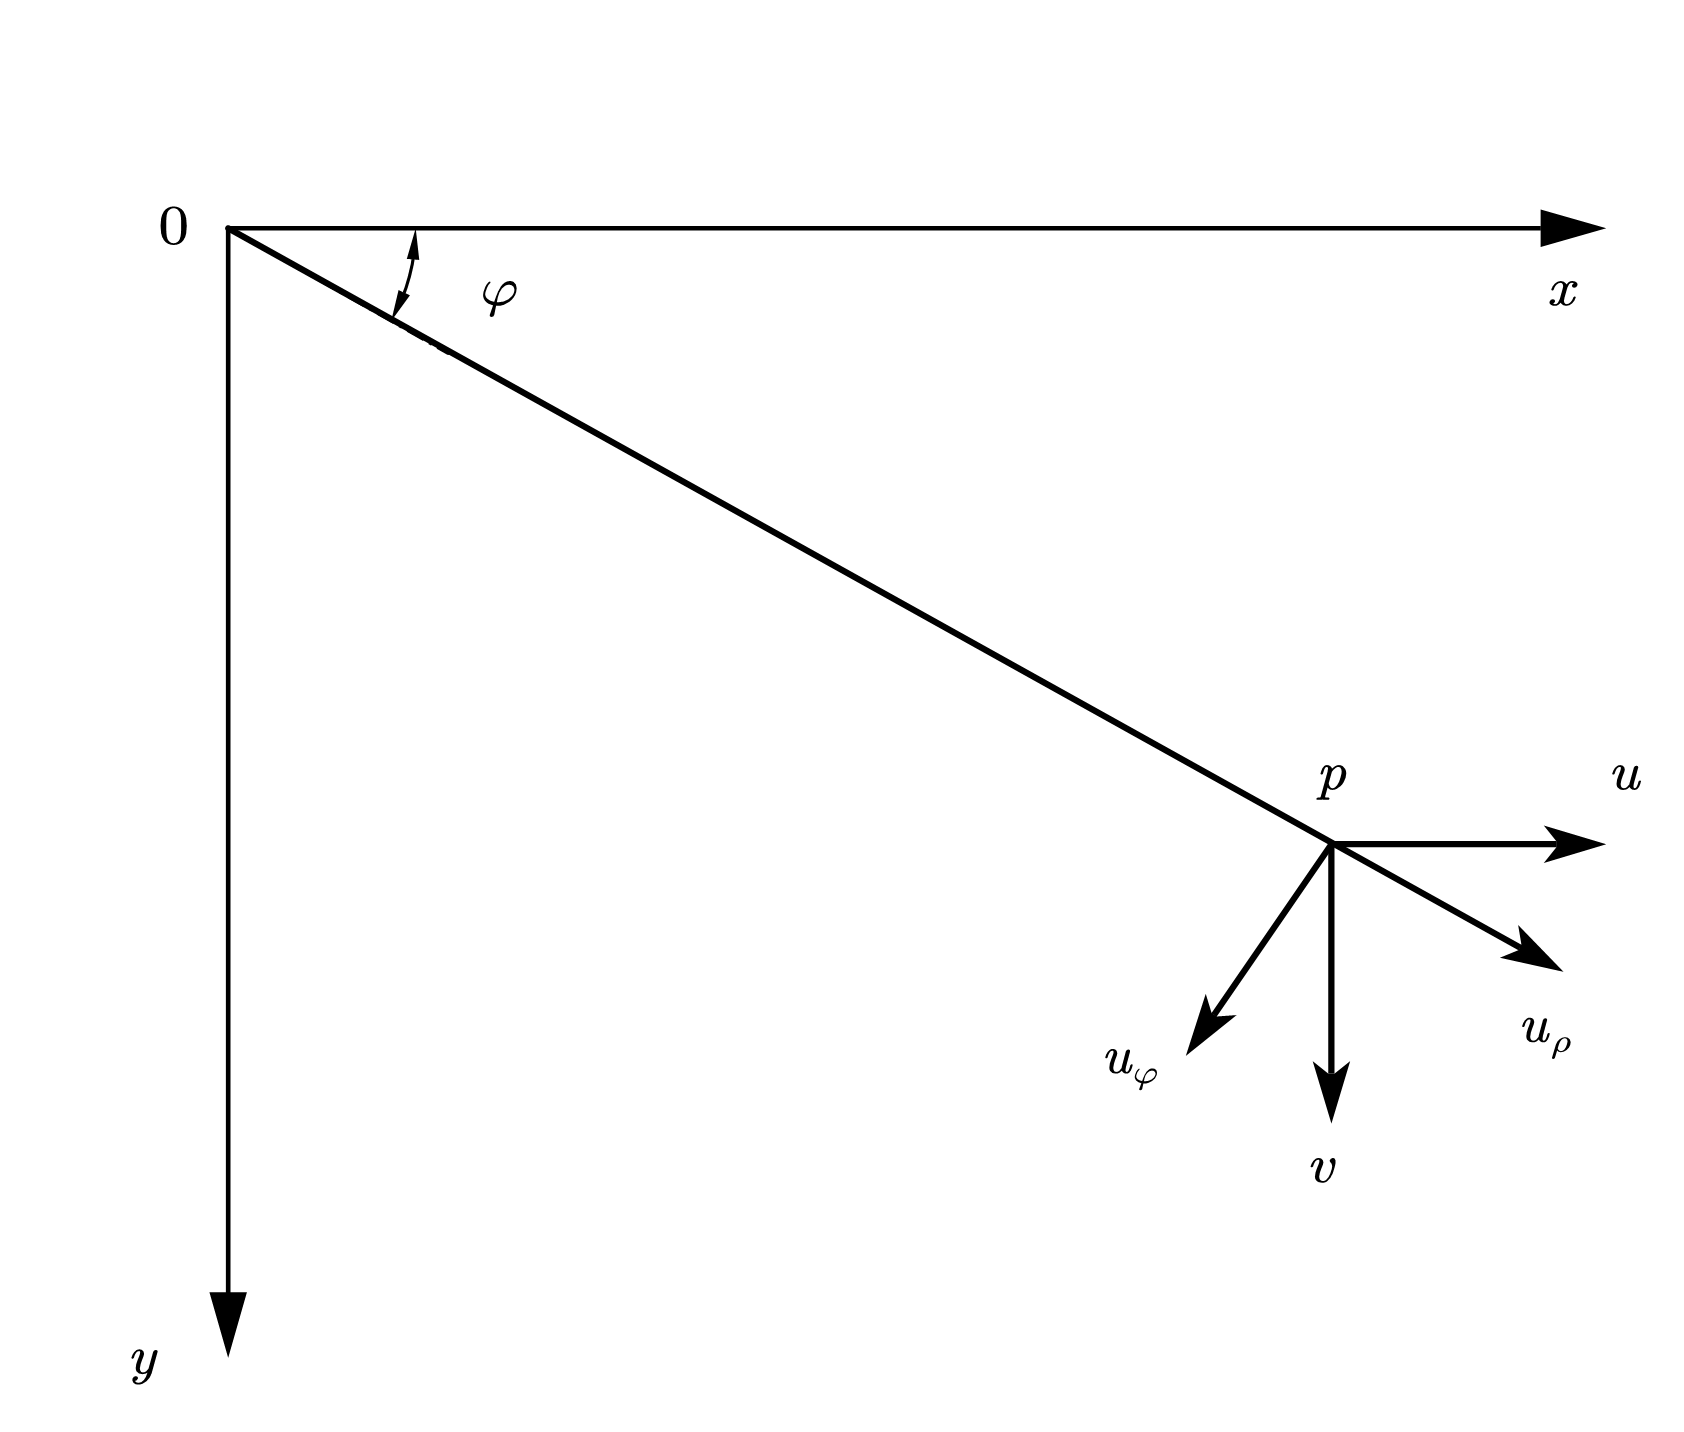
\includegraphics[scale=0.5]{figure/4-2.png}
\caption{}
\end{figure}
\begin{equation}
\begin{cases}
u_{\rho}=u\cos \varphi +v\sin \varphi\\
u_{\varphi}=-u\sin \varphi +v\cos \varphi\\
\end{cases}\Longrightarrow \left( \begin{array}{c}
u_{\rho}\\
u_{\varphi}\\
\end{array} \right) =\left[ \begin{matrix}
\cos \varphi&		\sin \varphi\\
-\sin \varphi&		\cos \varphi\\
\end{matrix} \right] 
,
	\left( \begin{array}{c}
u\\
v\\
\end{array} \right) =\left[ \begin{matrix}
\cos \varphi&		-\sin \varphi\\
\sin \varphi&		\cos \varphi\\
\end{matrix} \right] \left( \begin{array}{c}
u_{\rho}\\
u_{\varphi}\\
\end{array} \right) 
\end{equation}
\subsubsection{应力分量的坐标变换}
\begin{figure}[!h]
\centering
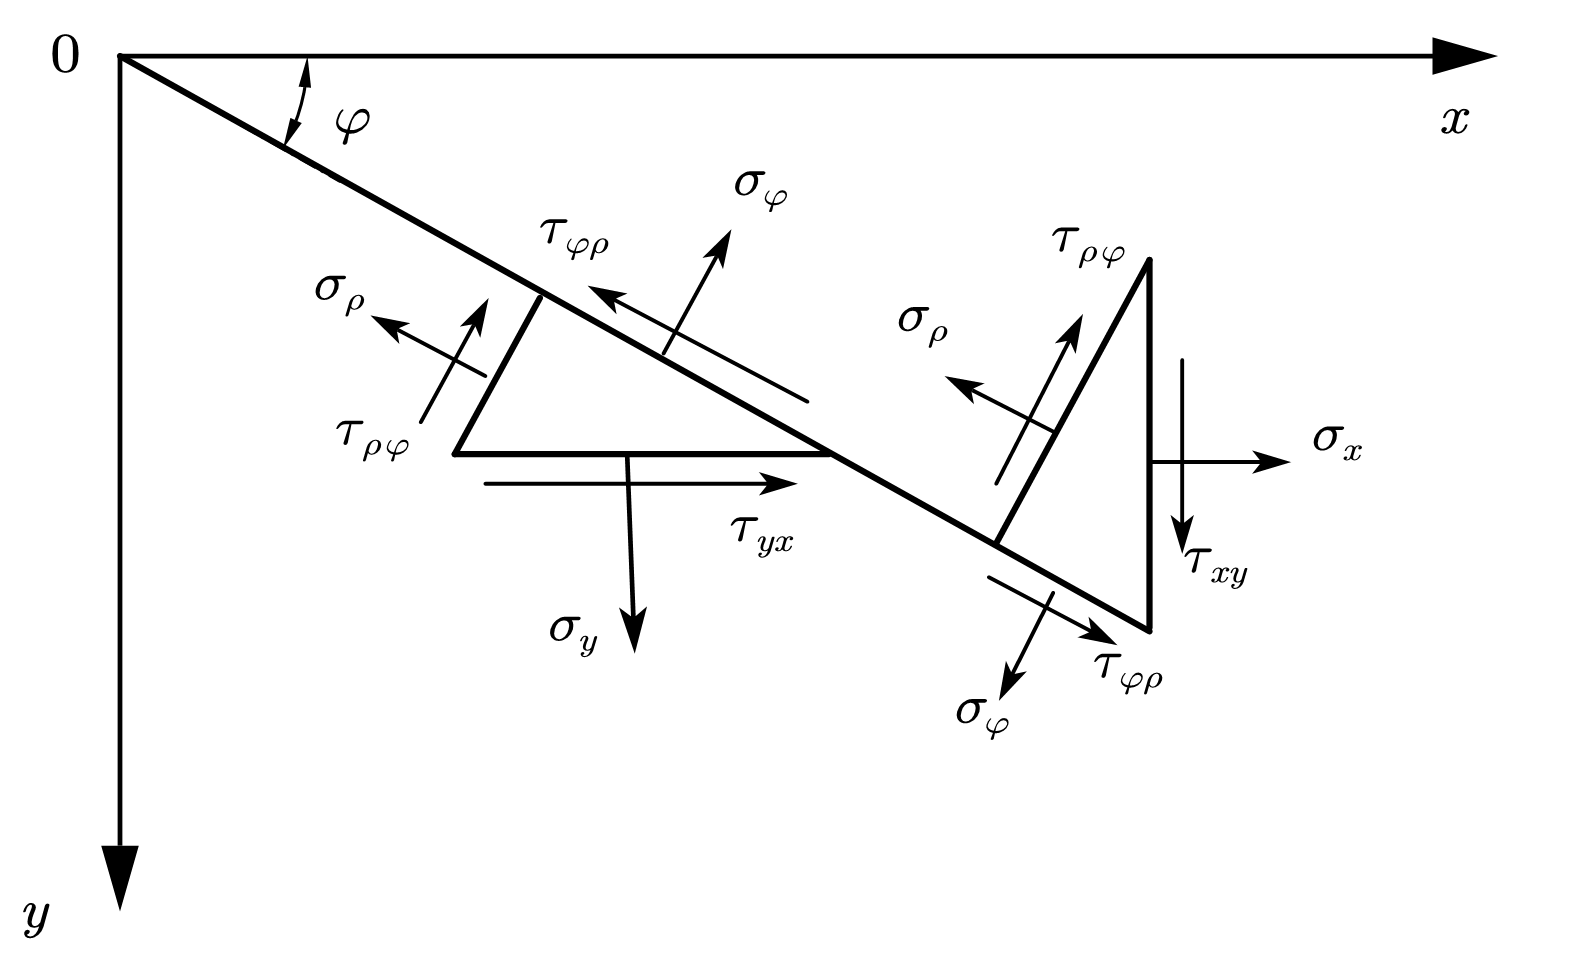
\includegraphics[scale=0.5]{figure/4-3.png}
\caption{}
\end{figure}
\begin{equation}
\begin{cases}
\sigma _x=\sigma _{\rho}\cos ^2\varphi +\sigma _{\varphi}\sin ^2\varphi -2\tau _{\rho \varphi}\sin \varphi \cos \varphi\\
\sigma _y=\sigma _{\rho}\sin ^2\varphi +\sigma _{\varphi}\cos ^2\varphi +2\tau _{\varphi \rho}\sin \varphi \cos \varphi\\
\tau _{xy}=\frac{\sigma _{\rho}-\sigma _{\varphi}}{2}\sin 2\varphi +\tau _{\rho \varphi}\cos 2\varphi\\
\end{cases}
\end{equation}
\begin{equation}
\begin{cases}
\sigma _x=\frac{\sigma _{\rho}+\sigma _{\varphi}}{2}+\frac{\sigma _{\rho}-\sigma _{\varphi}}{2}\cos 2\varphi -\tau _{\rho \varphi}\sin 2\varphi\\
\sigma _y=\frac{\sigma _{\rho}+\sigma _{\varphi}}{2}-\frac{\sigma _{\rho}-\sigma _{\varphi}}{2}\cos 2\varphi -\tau _{\rho \varphi}\sin 2\varphi\\
\tau _{xy}=\frac{\sigma _{\rho}-\sigma _{\varphi}}{2}\sin 2\varphi +\tau _{\rho \varphi}\cos 2\varphi\\
\end{cases}
\\
\end{equation}
\begin{equation}
\left[ \begin{matrix}
\sigma _x&		\tau _{xy}\\
\tau _{yx}&		\sigma _y\\
\end{matrix} \right] =\left[ \begin{matrix}
\cos \varphi&		\sin \varphi\\
-\sin \varphi&		\cos \varphi\\
\end{matrix} \right] \left[ \begin{matrix}
\sigma _{\rho}&		\tau _{\varphi \rho}\\
\tau _{\rho \varphi}&		\sigma _{\varphi}\\
\end{matrix} \right] \left[ \begin{matrix}
\cos \varphi&		\sin \varphi\\
-\sin \varphi&		\cos \varphi\\
\end{matrix} \right] ^T
\end{equation}
\begin{figure}[!h]
	\centering
	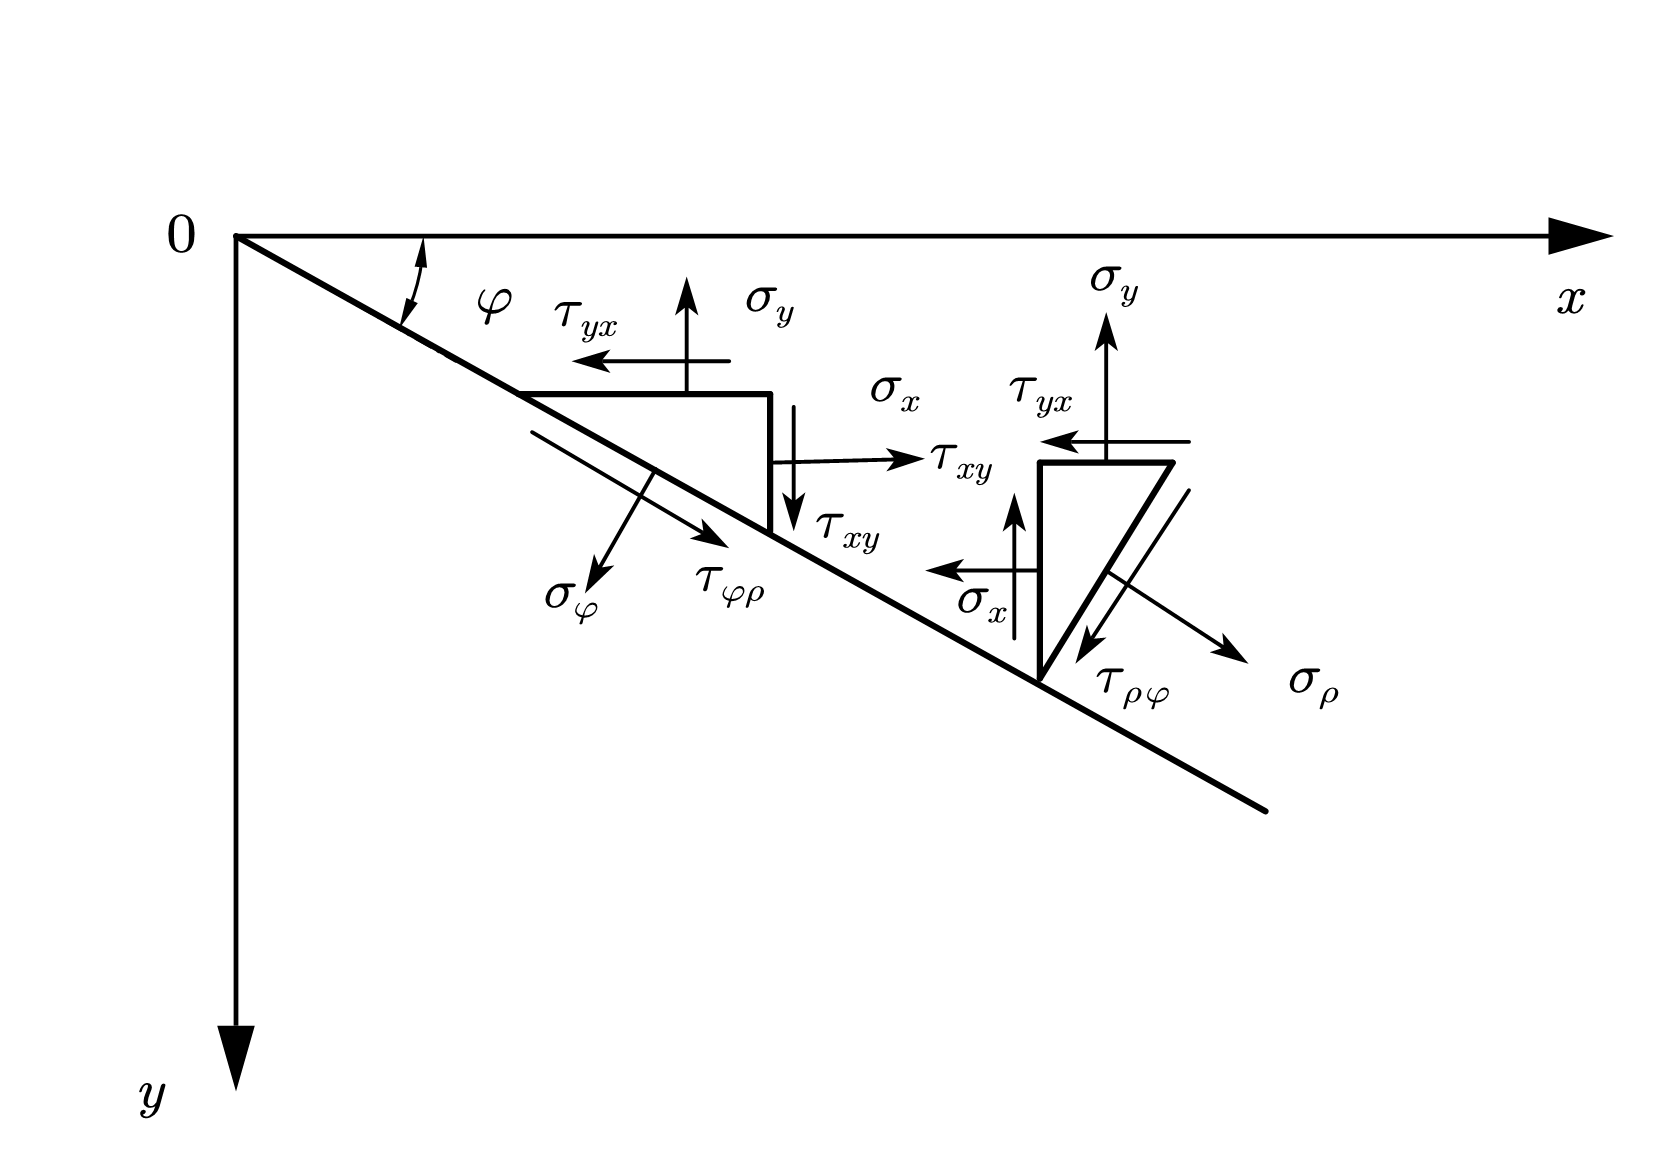
\includegraphics[scale=0.5]{figure/4-4.png}
	\caption{}
\end{figure}
\begin{equation}
\begin{cases}
\sigma _{\rho}=\sigma _x\cos ^2\varphi +\sigma _y\sin ^2\varphi +2\tau _{xy}\sin \varphi \cos \varphi\\
\sigma _{\varphi}=\sigma _x\sin ^2\varphi +\sigma _y\cos ^2\varphi -2\tau _{xy}\sin \varphi \cos \varphi\\
\tau _{\rho \varphi}=\left( \sigma _y-\sigma _x \right) \sin \varphi \cos \varphi +\tau _{xy}\left( \cos ^2\varphi -\sin ^2\varphi \right)\\
\end{cases}
\end{equation}
\begin{equation}
\begin{cases}
\sigma _{\rho}=\frac{\sigma _x+\sigma _y}{2}+\frac{\sigma _x-\sigma _y}{2}\cos 2\varphi +\tau _{xy}\sin 2\varphi\\
\sigma _{\varphi}=\frac{\sigma _x+\sigma _y}{2}-\frac{\sigma _x-\sigma _y}{2}\cos 2\varphi -\tau _{xy}\sin 2\varphi\\
\tau _{\varphi \rho}=\frac{\sigma _x-\sigma _y}{2}\sin 2\varphi +\tau _{xy}\cos 2\varphi\\
\end{cases}
\end{equation}
\begin{equation}
\left[ \begin{matrix}
\sigma _{\rho}&		\tau _{\varphi \rho}\\
\tau _{\rho \varphi}&		\sigma _{\varphi}\\
\end{matrix} \right] =\left[ \begin{matrix}
\cos \varphi&		\sin \varphi\\
-\sin \varphi&		\cos \varphi\\
\end{matrix} \right] ^T\left[ \begin{matrix}
\sigma _x&		\tau _{xy}\\
\tau _{yx}&		\sigma _y\\
\end{matrix} \right] \left[ \begin{matrix}
\cos \varphi&		\sin \varphi\\
-\sin \varphi&		\cos \varphi\\
\end{matrix} \right]
\end{equation}
\subsection{极坐标中的应力函数与相容方程}
当$f_{\rho}=f_{\varphi}=0$时:
\begin{equation}\begin{cases}
\sigma _{\rho}=\frac{1}{\rho}\frac{\partial \varPhi}{\partial \rho}+\frac{1}{\rho ^2}\frac{\partial ^2\varPhi}{\partial \varphi ^2}\\
\sigma _{\varphi}=\frac{\partial ^2\varPhi}{\partial \rho ^2}\\
\tau _{\rho \varphi}=-\frac{\partial}{\partial \rho}\left( \frac{1}{\rho}\frac{\partial \varPhi}{\partial \varphi} \right)\\
\end{cases}
\\
\end{equation}
\subsubsection{相容方程}
\begin{equation}
\left( \frac{\partial ^2}{\partial \rho ^2}+\frac{1}{\rho}\frac{\partial}{\partial \rho}+\frac{1}{\rho ^2}\frac{\partial ^2}{\partial \varphi ^2} \right)^2 \varPhi =0
\end{equation}
\subsection{轴对称应力和相容的位移}
所谓轴对称问题,是指物体几何形状或某物理量是绕某一轴对称的,凡通过此轴的任何面均为对称面。如果该物体所受外部荷载也对称于该轴,那么相应所产生的应力也必对称该轴。
\\
令$\varPhi =\varPhi \left( \rho \right) $
\begin{equation}
\sigma _{\rho}=\frac{1}{\rho}\frac{d\varPhi}{d\rho}\,\,,     \sigma _{\varphi}=\frac{d^2\varPhi}{d\rho ^2},     \tau _{\rho \varphi}=0
\end{equation}
\begin{equation}
\left( \frac{d^2}{d\rho ^2}+\frac{1}{\rho}\frac{d}{d\rho} \right) ^2\varPhi =0
\end{equation}
即
\begin{equation}
\varPhi =A\ln \rho +B\rho ^2\ln \rho +C\rho ^2+D
\end{equation}
应力分量
\begin{equation}
\begin{cases}
\sigma _{\rho}=\frac{A}{\rho ^2}+B\left( 1+2\ln \rho \right) +2C\\
\sigma _{\varphi}=-\frac{A}{\rho ^2}+B\left( 3+2+\ln \rho \right) +2C\\
\tau _{\rho \varphi}=0\\
\end{cases}
\end{equation}
代入物理方程和几何方程可得位移分量
\begin{equation}
\begin{cases}
u_{\rho}=\frac{1}{E}\left[ -\left( 1+\mu \right) \frac{A}{\rho}+2\left( 1-\mu \right) B\rho \left( \ln \rho -1 \right) +\left( 1-3\mu \right) B\rho +2\left( 1-\mu \right) C\rho \right] +I\cos \varphi +K\sin \varphi\\
u_{\varphi}=\frac{4B\rho \varphi}{E}+H\rho -I\sin \varphi +K\cos \varphi\\
\end{cases}
\end{equation}
\begin{enumerate}
\item 在轴对称应力条件下,应力、应变和位移的通解,适用于任何轴对称应力问题。
\item 在轴对称应力条件下,应变也是轴对称的,但位移不一定是轴对称的。
\item 实现轴对称应力的条件是:物体形状、体力和面力应是轴对称的。
\item 轴对称应力及对应的位移的通解已满足相容方程,它们还需满足边界条件及多连体中的位移单值条件,并由此求出系数A、B、C。
\end{enumerate}
\begin{note}
欧拉方程:
\[x^ny^{\left( n \right)}+P_1x^{n-1}y^{\left( n-1 \right)}+\cdots +P_{n-1}xy'+P_ny=0\]
特征方程为:
\[\left[ k\left( k-1 \right) \cdots \left( k-n+1 \right) +P_1\left[ k\left( k-1 \right) \cdots \left( k-n+2 \right) \right] +\cdots +P_{n-1}k+P_n \right] =0\]
关于$K$的$n$次代数方程,可解得n个特征根$k_1\text{、}k_2\text{、}\cdots k_n$
\begin{enumerate}
\item 当它们是互不相等的实根时,通解具有幂函数的形式
\[y=C_1x^{k_1}+C_2x^{k_2}+\cdots +C_nx^{k_n}\]
\item 每当出现重根时,每多一重根,就多乘一个$\ln x$\\
如:当$k_1$为$m\left( m<n \right) $重根时,通解为
\[y=C_1x^{k_1}+C_2x^{k_2}\ln x+\cdots +C_mx^{k_1}\ln ^{m-1}x+C_{m+1}x^{k_{m+1}}+\cdots +C_nx^{k_n}\]
\item 出现共轭复根时,则虚部是三角函数因子\\
如: 当$k_{1,2}=\alpha \pm i\beta $,通解为
\[y=C_1x^{\alpha}\cos \left( \beta \ln x \right) +C_2x^{\alpha}\sin \left( \beta \ln x \right) +C_3x^{k_3}+\cdots +C_nx^{k_n}\]
\item 当出现复重根,则实部要多乘因子$\ln x$\\
如:$k_{1,2}=\alpha \pm i\beta $为$m\left( m<\frac{n}{2} \right) $重共轭复根时,通解为
\begin{align*}
	y
	= & \left[ C_1x^{\alpha}+C_2x^{\alpha}\ln x+\cdots +C_mx^{\alpha}\ln ^{m-1}x \right] \cos \left( \beta \ln x \right) +\\
	&\left[ C_{m+1}x^{\alpha}+C_{m+2}x^{\alpha}\ln x+\cdots +C_{2m}x^{\alpha}\ln ^{m-1}x \right] \sin \left( \beta \ln x \right) +\\
	&C_{2m+1}x^{k_{2m+1}}+\cdots +C_nx^{k_n}
\end{align*}
\end{enumerate}
\end{note}

\begin{example}
试求解平面轴对称应力问题的相容方程\[\rho ^4\varPhi ^{\left( 4 \right)}+2\rho ^3\varPhi ^{\left( 3 \right)}-\rho ^2\varPhi ''+\rho \varPhi '=0\]
\end{example}
	\begin{remark}
	特征方程:
	\[k\left( k-1 \right) \left( k-2 \right) \left( k-3 \right) +2k\left( k-1 \right) \left( k-2 \right) -k\left( k-1 \right) +k=0\]
	解得:$$k_{1,2}=0,k_{3,4}=2$$\\
	得:$$\varPhi =A\ln \rho +B\rho ^2\ln \rho +C\rho ^2+D$$
	\end{remark}

\begin{example}
试求解如下的常微分方程
\[\rho ^4f^{\left( 4 \right)}\left( \rho \right) +2\rho ^3f'''\left( \rho \right) -9\rho ^2f''\left( \rho \right) +9\rho f'\left( \rho \right) =0\]
\end{example}
	\begin{remark}
		特征方程:
		\[k\left( k-1 \right) \left( k-2 \right) \left( k-3 \right) +2k\left( k-1 \right) \left( k-2 \right) -9k\left( k-1 \right) +9k=0\]
		解得:\[k_1=4,k_2=2,k_3=0,k_4=-2\]
		得:\[f\left( \rho \right) =A\rho ^4+B\rho ^2+C+D\rho ^{-2}\]
	\end{remark}
\subsection{圆环或圆筒受均布压力}
\begin{example}
设有圆环(平面应力问题)或圆筒(平面应变问题)受均匀内压力$q_1$,和外压力$q_2$作用;内半径为$r$;外半径为$R$。试求应力分量;位移分量。
\end{example}
\begin{figure*}[!h]
	\centering
	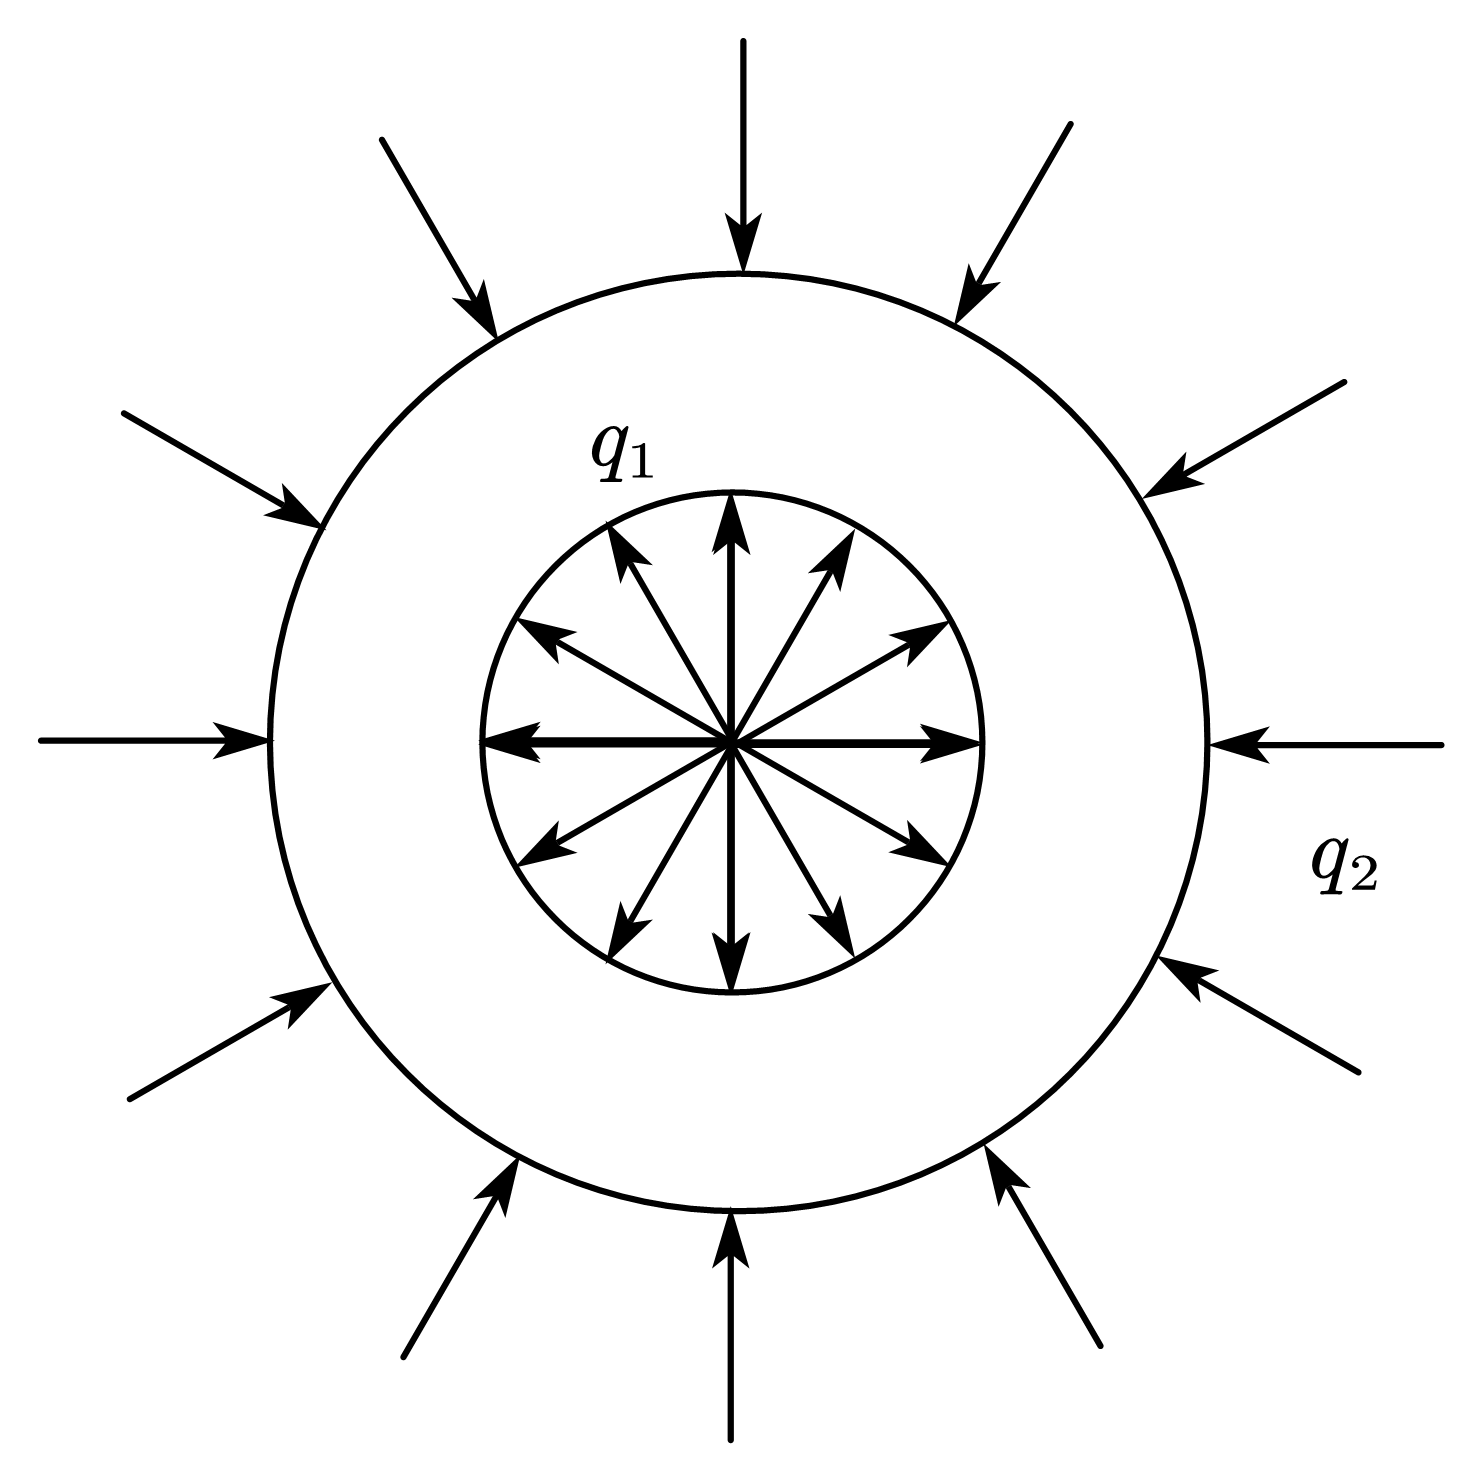
\includegraphics[scale=0.3]{figure/4-5.png}
\end{figure*}
	\begin{remark}
		轴对称应力问题的应力通解:
		\begin{equation*}
			\begin{cases}
			\sigma _{\rho}=\frac{A}{\rho ^2}+B\left( 1+2\ln \rho \right) +2C\\
			\sigma _{\varphi}=-\frac{A}{\rho ^2}+B\left( 3+2+\ln \rho \right) +2C\\
			\tau _{\rho \varphi}=0\\
			\end{cases}
		\end{equation*}
		应力边界条件:
		\begin{equation*}
			\begin{cases}
			\left( \sigma _{\rho} \right) _{\rho =r}=-q_1\\
			\left( \sigma _{\rho} \right) _{\rho =R}=-q_2\\
			\left( \tau _{\rho \varphi} \right) _{\rho =r}=\left( \tau _{\rho \varphi} \right) _{\rho =R}=0\\
			\end{cases}\Longrightarrow \left\{ \begin{array}{c}
			\frac{A}{r^2}+B\left( 1+2\ln r \right) +2C=-q_1\\
			\frac{A}{R^2}+B\left( 1+2\ln r \right) +2C=-q_2\\
			\end{array} \right. 
		\end{equation*}
		圆环或圆筒具有贯穿孔洞,为多连体,故需进一步考虑位移单值条件:
		由\[u_{\varphi}=\frac{4B\rho \varphi}{E}+H\rho -I\sin \varphi +K\cos \varphi \]
		考虑$\left( \rho ,\varphi \right) \text{和}\left( \rho ,\varphi +2\pi \right) $同一点只能有一确定的位移,故$B=0$。
		则:\[\begin{cases}
		A=\frac{r^2R^2\left( q_2-q_1 \right)}{R^2-r^2}\\
		C=\frac{q_1r^2-q_2R^2}{R^2-r^2}\\
		\end{cases}\]
		得(拉梅的解答):\[\begin{cases}
		\sigma _{\rho}=\frac{\frac{R^2}{\rho ^2}-1}{\frac{R^2}{r^2}-1}q_1-\frac{1-\frac{r^2}{\rho ^2}}{1-\frac{r^2}{R^2}}q_2\\
		\sigma _{\varphi}=\frac{\frac{R^2}{\rho ^2}+1}{\frac{R^2}{r^2}-1}q_1-\frac{1+\frac{r^2}{\rho ^2}}{1-\frac{r^2}{R^2}}q_2\\
		\end{cases}\]
	\end{remark}

\begin{example}
轴对称应力条件下的应力和位移的通解,可以应用于各种应力边界条件和位移边界条件的情形,试考虑下列圆环或圆筒的问题应如何求解
\begin{enumerate}
	\item 内边界受均布压力$q_1$作用,而外边界为固定边.
	\item 外边界受均布压力$q_2$作用,而内边界为固定边.
	\item 外边界受到强迫的均匀位移$u_{\rho}=-\varDelta $,而内边界为自由边(如车辆的轮毂的作用.
	\item 内边界受到强迫的均匀位移$u_{\rho}=\varDelta $,而外边界为自由边.
\end{enumerate}
\end{example}
		\begin{remark}
			\quad \\
			\begin{enumerate}
				\item 应力边界条件:\[\begin{cases}
				\left( \sigma _{\rho} \right) _{\rho =r}=-q_1\\
				\left( \tau _{\rho \varphi} \right) _{\rho =r}=0\\
				\end{cases}\Longrightarrow \frac{A}{r ^2}+2C=-q_1\]
				位移边界条件:\[\begin{cases}
				\left( u_{\rho} \right) _{\rho =R}=0\\
				\left( u_{\varphi} \right) _{\rho =R}=0\\
				\end{cases}\Longrightarrow \begin{cases}
				H=I=K=0\\
				-\left( 1+\mu \right) \frac{A}{R}+2\left( 1-\mu \right) CR=0\\
				\end{cases}\]
				
				\item 应力边界条件:\[\begin{cases}
				\left( \sigma _{\rho} \right) _{\rho =R}=-q_2\\
				\left( \tau _{\rho \varphi} \right) _{\rho =R}=0\\
				\end{cases}\Longrightarrow \frac{A}{R^2}+2C=-q_2\]
				位移边界条件:\[\begin{cases}
				\left( u_{\rho} \right) _{\rho =r}=0\\
				\left( u_{\varphi} \right) _{\rho =r}=0\\
				\end{cases}\Longrightarrow \begin{cases}
				H=I=K=0\\
				-\left( 1+\mu \right) \frac{A}{r}+2\left( 1-\mu \right) Cr=0\\
				\end{cases}\]
				
				\item 应力边界条件:\[\begin{cases}
				\left( \sigma _{\rho} \right) _{\rho =r}=0\\
				\left( \tau _{\rho \varphi} \right) _{\rho =r}=0\\
				\end{cases}\Longrightarrow \frac{A}{r^2}+2C=0\]
				位移边界条件:\[\begin{cases}
				\left( u_{\rho} \right) _{\rho =R}=-\varDelta\\
				\left( u_{\varphi} \right) _{\rho =R}=0\\
				\end{cases}\Longrightarrow \begin{cases}
				H=I=K=0\\
				-\left( 1+\mu \right) \frac{A}{R}+2\left( 1-\mu \right) CR=-E\varDelta\\
				\end{cases}\]
				
				\item 应力边界条件:\[\begin{cases}
				\left( \sigma _{\rho} \right) _{\rho =R}=0\\
				\left( \tau _{\rho \varphi} \right) _{\rho =R}=0\\
				\end{cases}\Longrightarrow \frac{A}{R^2}+2C=0\]
				位移边界条件:$$\begin{cases}
					\left( u_{\rho} \right) _{\rho =r}=-\varDelta\\
					\left( u_{\varphi} \right) _{\rho =r}=0\\
				\end{cases}\Longrightarrow \begin{cases}
					H=I=K=0\\
					-\left( 1+\mu \right) \frac{A}{r}+2\left( 1-\mu \right) Cr=-E\varDelta\\
				\end{cases}$$
			\end{enumerate}
		\end{remark}
	
\begin{example}
	实心圆盘在$\rho = r$的圆周上受有均布压力$q$的作用,试求其应力分量。
\end{example}
\begin{figure*}[!h]
	\centering
	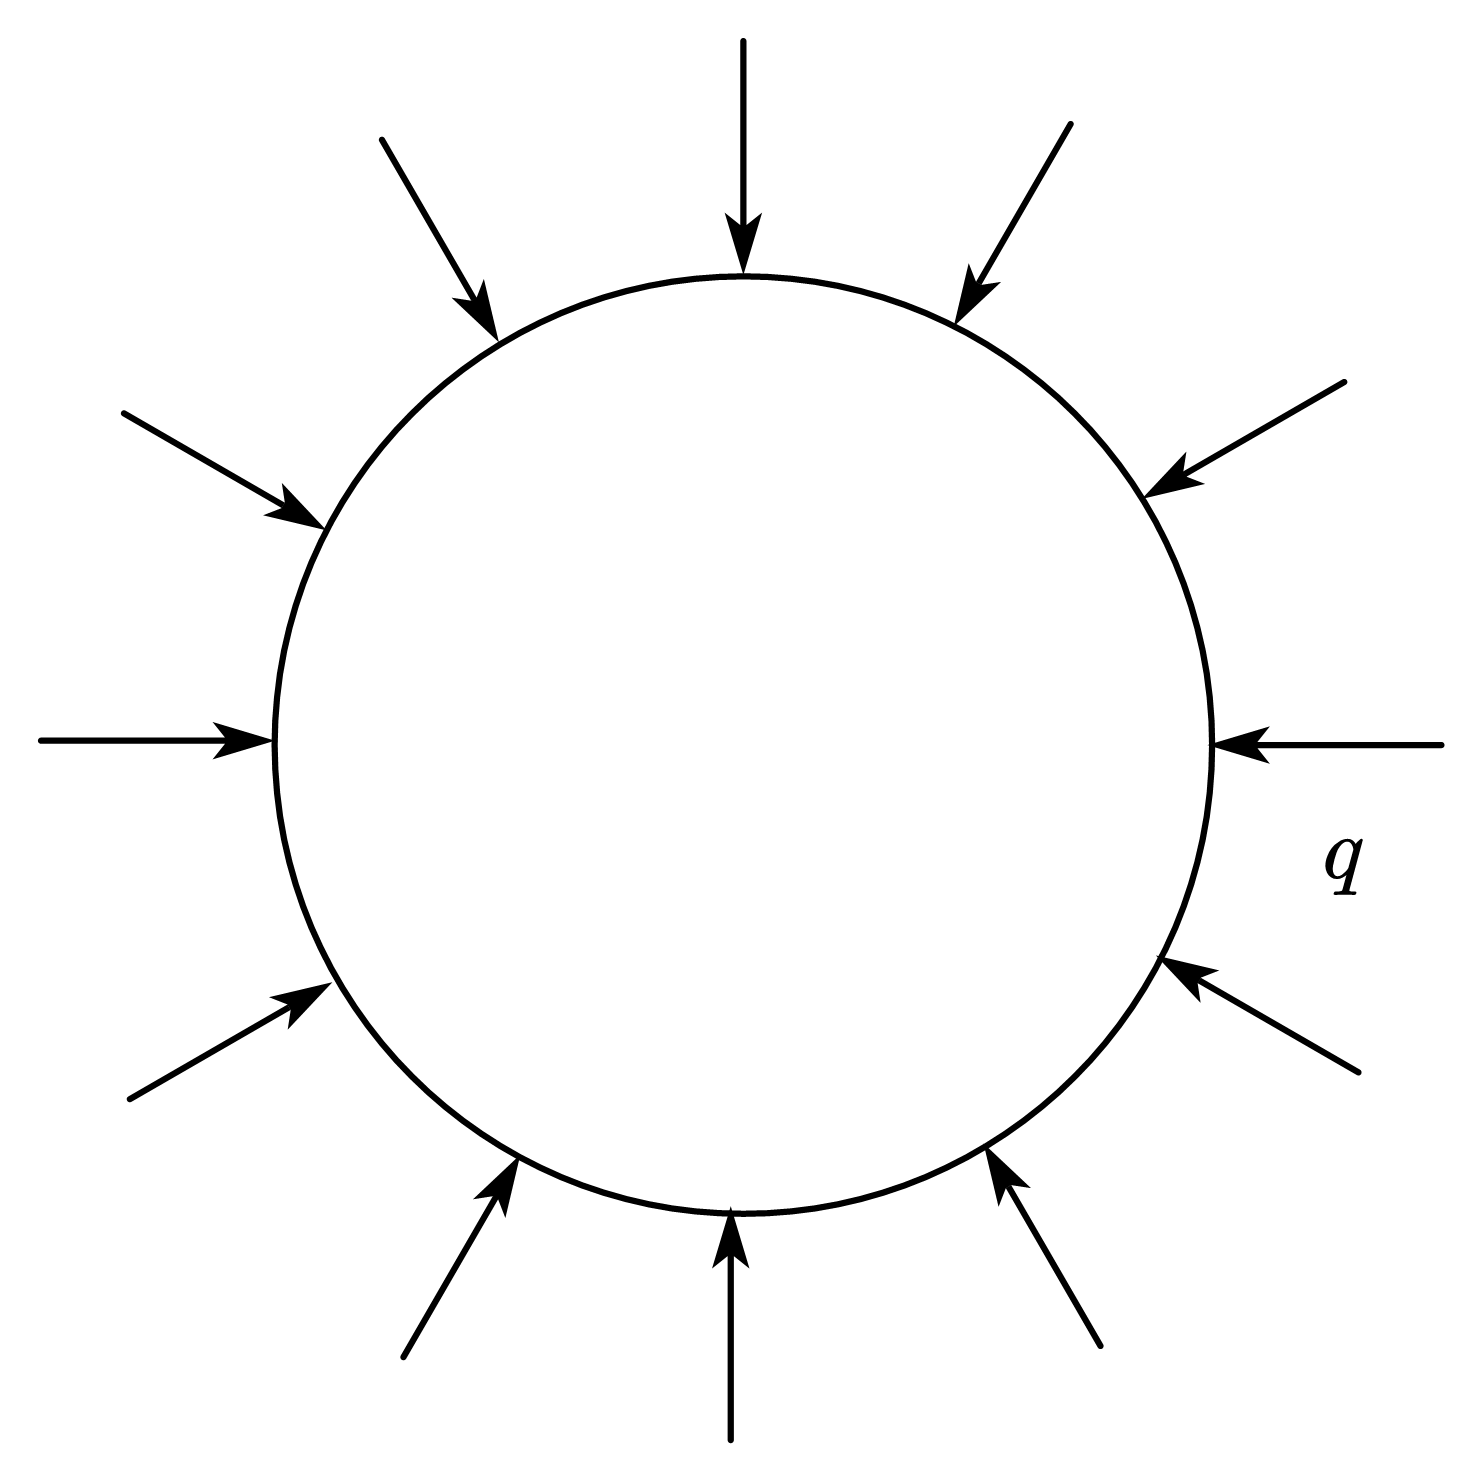
\includegraphics[scale=0.25]{figure/4-6.png}
\end{figure*}
	\begin{remark}
		平面轴对称应用问题,应力通解为:
		\begin{equation*}
		\begin{cases}
		\sigma _{\rho}=\frac{A}{\rho ^2}+B\left( 1+2\ln \rho \right) +2C\\
		\sigma _{\varphi}=-\frac{A}{\rho ^2}+B\left( 3+2\ln \rho \right) +2C\\
		\tau _{\rho \varphi}=0\\
		\end{cases}
		\end{equation*}
		应力的有界性,圆盘中心处(即$\rho=0$)处的应力值应当有界,不能是无限大的故$A=B=0$
		\\
		应力边界条件:\[\begin{cases}
		\left( \sigma _{\rho} \right) _{\rho =r}=-q\\
		\left( \tau _{\rho \varphi} \right) _{\rho =r}=0\\
		\end{cases}\Longrightarrow C=-\frac{q}{2}\]
		故实心圆盘的应力解答:\[\begin{cases}
		\sigma _{\rho}=\sigma _{\varphi}=-q\\
		\tau _{\rho \varphi}=0\\
		\end{cases}\]
	\end{remark}

\subsection{压力隧洞}
问题描述:圆筒埋在无限大弹性体中,受有均布内压力$q$,设圆筒和无限大弹性体的弹性常数分别为$E,\mu,\text{和}E',\mu'$\\
\hspace*{2em}问题本质:本题是两个圆筒的接触问题,两个圆筒均为轴对称问题(平面应变问题),因为不符合均匀性假定,必须分别采用两个轴对称解答。
\begin{figure}[H]
	\centering
	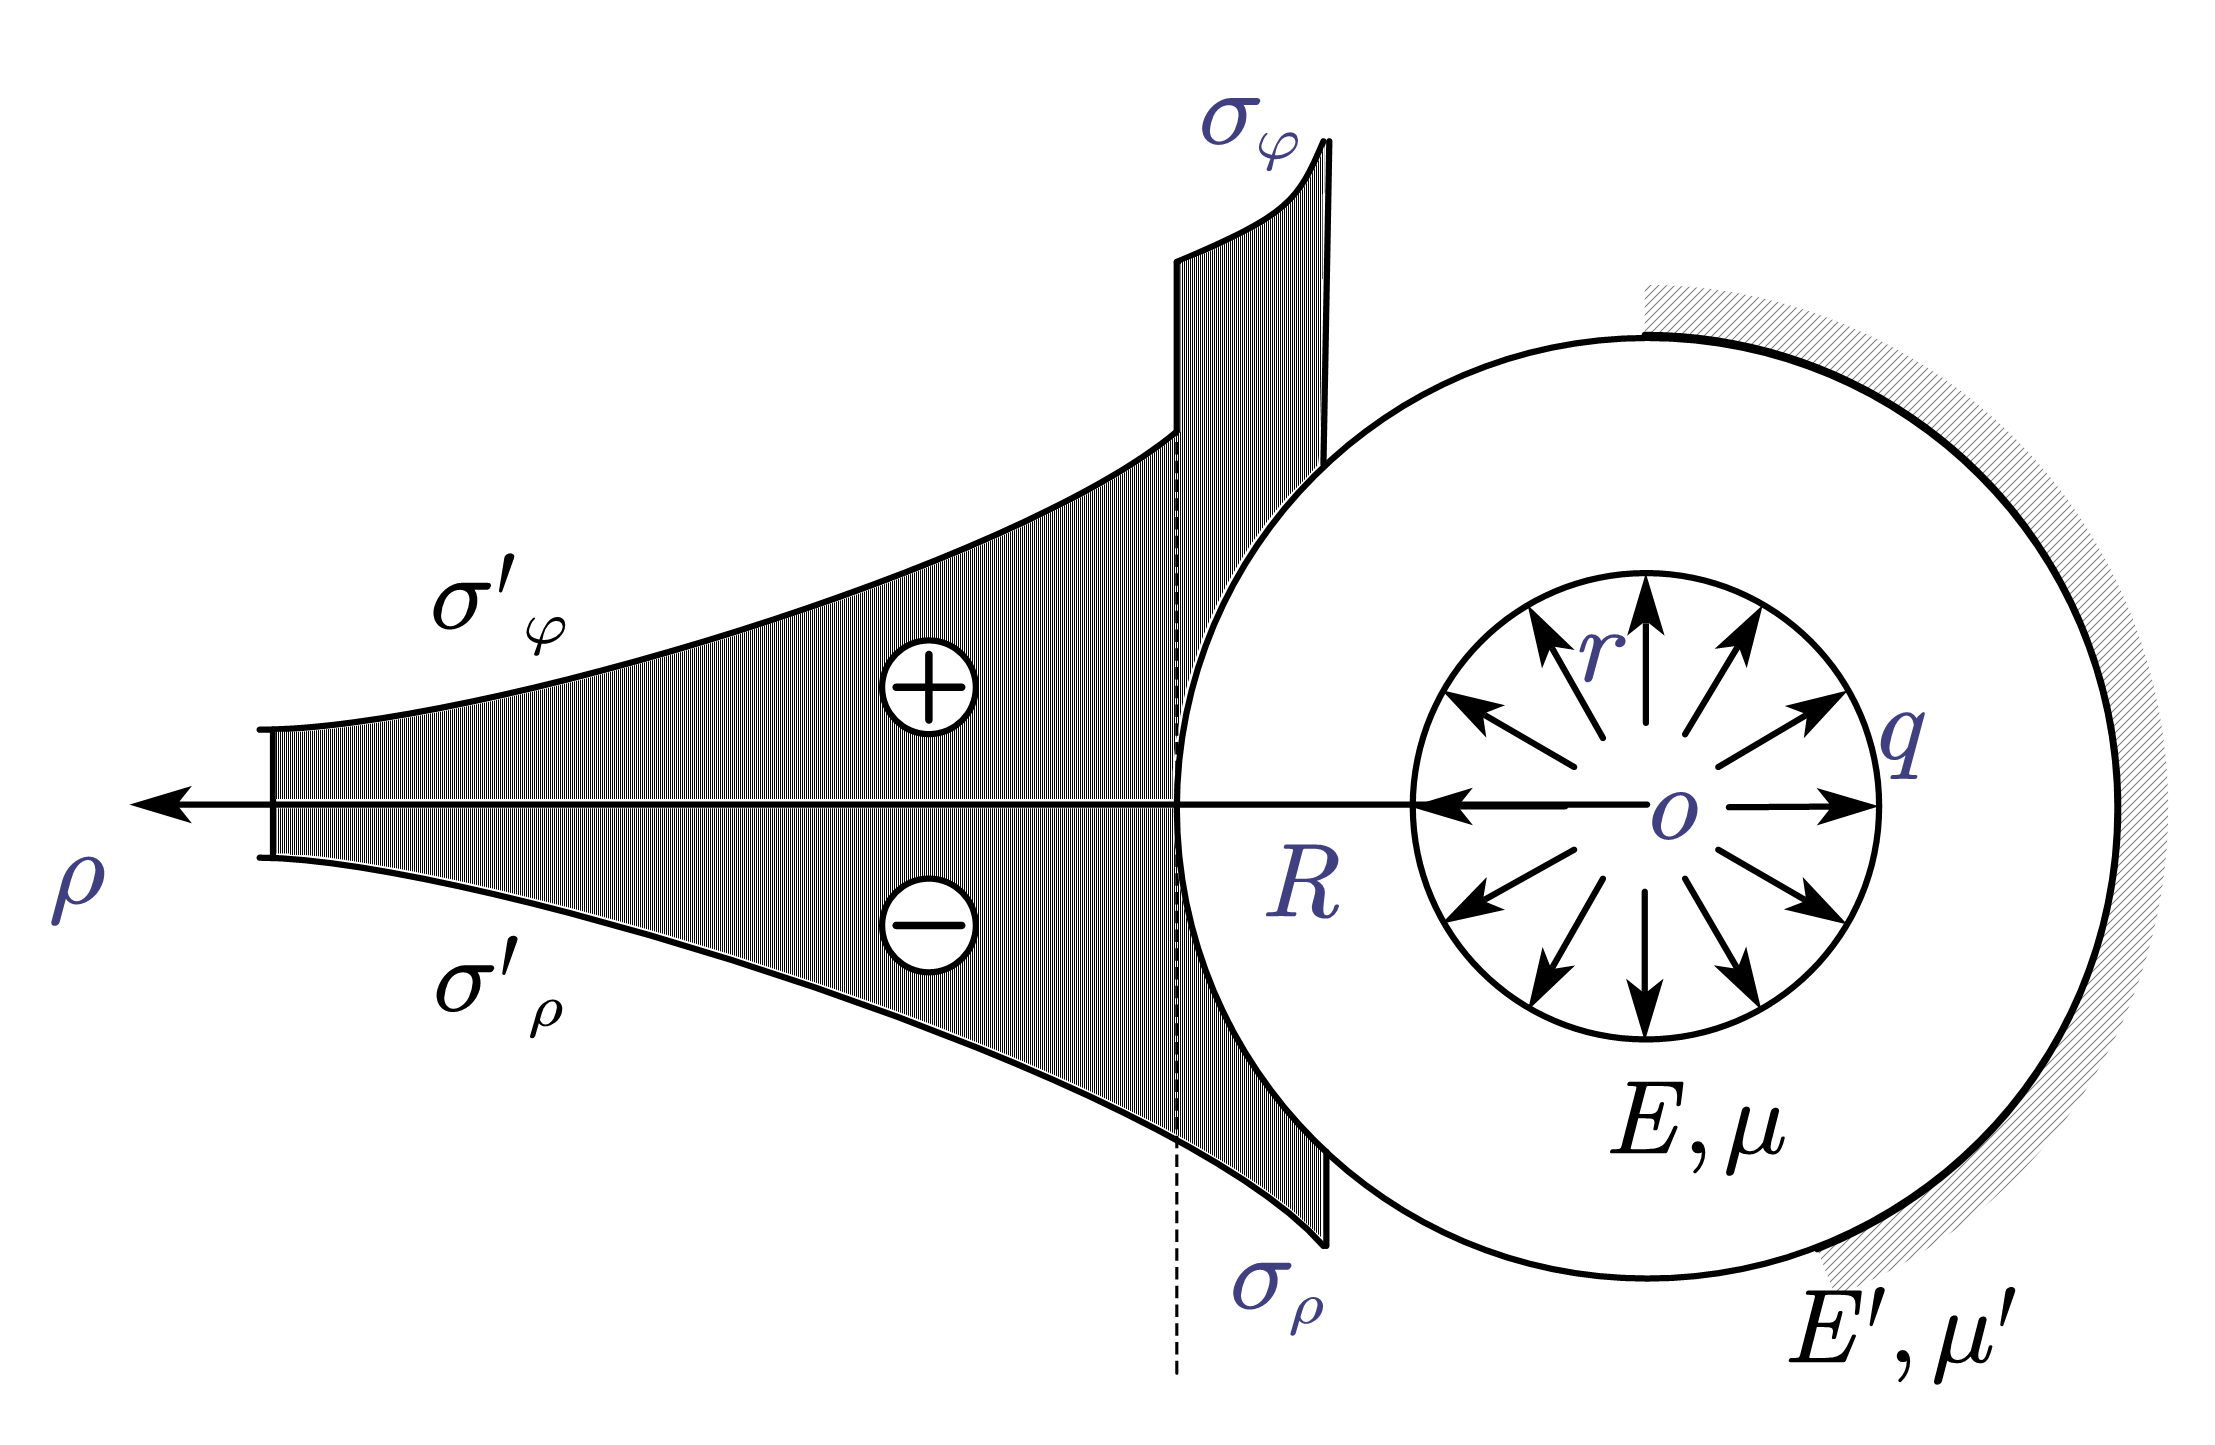
\includegraphics[scale=0.5]{figure/4-7.png}
	\caption{$n<1$}
\end{figure}
不管是内圆筒还是外弹性体,都有贯穿孔道,属于多连体,故需要考虑位移单值条件有$B=0,B'=0$。\\
内圆筒应力表达式:\[\begin{cases}
\sigma _{\rho}=\frac{A}{\rho ^2}+2C\\
\sigma _{\varphi}=-\frac{A}{\rho ^2}+2C\\
\end{cases}\]
无限大弹性体应力表达式:\[\begin{cases}
\sigma '_{\rho}=\frac{A'}{\rho ^2}+2C'\\
\sigma '_{\varphi}=-\frac{A'}{\rho ^2}+2C'\\
\end{cases}\]
根据圣维南原理,离内圆筒的无穷远处的应力应为零。并且圆筒和无限大弹性体的接触面上的应力应当相等
则边界条件为:\[\begin{cases}
\left( \sigma _{\rho} \right) _{\rho =r}=-q\\
\left( \sigma '_{\rho} \right) _{\rho \rightarrow \infty}=0\\
\left( \sigma _{\rho} \right) _{\rho =R}=\left( \sigma '_{\rho} \right) _{\rho =R}\\
\end{cases}\]
即:\[\begin{cases}
\frac{A}{r^2}+2C=-q\\
C'=0\\
\frac{A}{R^2}+2C=\frac{A'}{R^2}+2C'\\
\end{cases}\]
在接触面上圆筒和无限大弹性体应当具有相同的位移,得:\[\left( u_{\rho} \right) _{\rho =R}=\left( u'_{\rho} \right) _{\rho =R}\]
即:\[\frac{1+\mu}{E}\left[ 2\left( 1-2\mu \right) CR-\frac{A}{R} \right] +I\cos \varphi +K\sin \varphi =\frac{1+\mu '}{E'}\left[ 2\left( 1-2\mu ' \right) C'R-\frac{A'}{R} \right] +I'\cos \varphi +K'\sin \varphi \]
因为在接触面的任意一点都要满足上式,则有:\[\frac{1+\mu}{E}\left[ 2\left( 1-2\mu \right) CR-\frac{A}{R} \right] =\frac{1+\mu '}{E'}\left[ 2\left( 1-2\mu ' \right) C'R-\frac{A'}{R} \right] \]
令$n=\frac{E'\left( 1+\mu \right)}{E\left( 1+\mu ' \right)}$:
综合方程,联立可得:
\begin{equation}
\begin{cases}
\sigma _{\rho}=-q\frac{\left[ 1+\left( 1-2\mu \right) n \right] \frac{R^2}{\rho ^2}-\left( 1-n \right)}{\left[ 1+\left( 1-2\mu \right) n \right] \frac{R^2}{r^2}-\left( 1-n \right)}\\
\sigma _{\rho}=q\frac{\left[ 1+\left( 1-2\mu \right) n \right] \frac{R^2}{\rho ^2}+\left( 1-n \right)}{\left[ 1+\left( 1-2\mu \right) n \right] \frac{R^2}{r^2}-\left( 1-n \right)}\\
\sigma _{\rho}'=-\sigma _{\varphi}'=-q\frac{2\left( 1-\mu \right) n\frac{R^2}{\rho ^2}}{\left[ 1+\left( 1-2\mu \right) n \right] \frac{R^2}{r^2}-\left( 1-n \right)}\\
\end{cases}
\end{equation}

\begin{example}
设有一刚体,具有半径$R$圆柱形孔道,孔道内放置外半径为$R$,内半径为$r$的圆筒,圆筒受均布压力q,试求出圆筒的应力。
\end{example}
\begin{figure*}[!h]
	\centering
	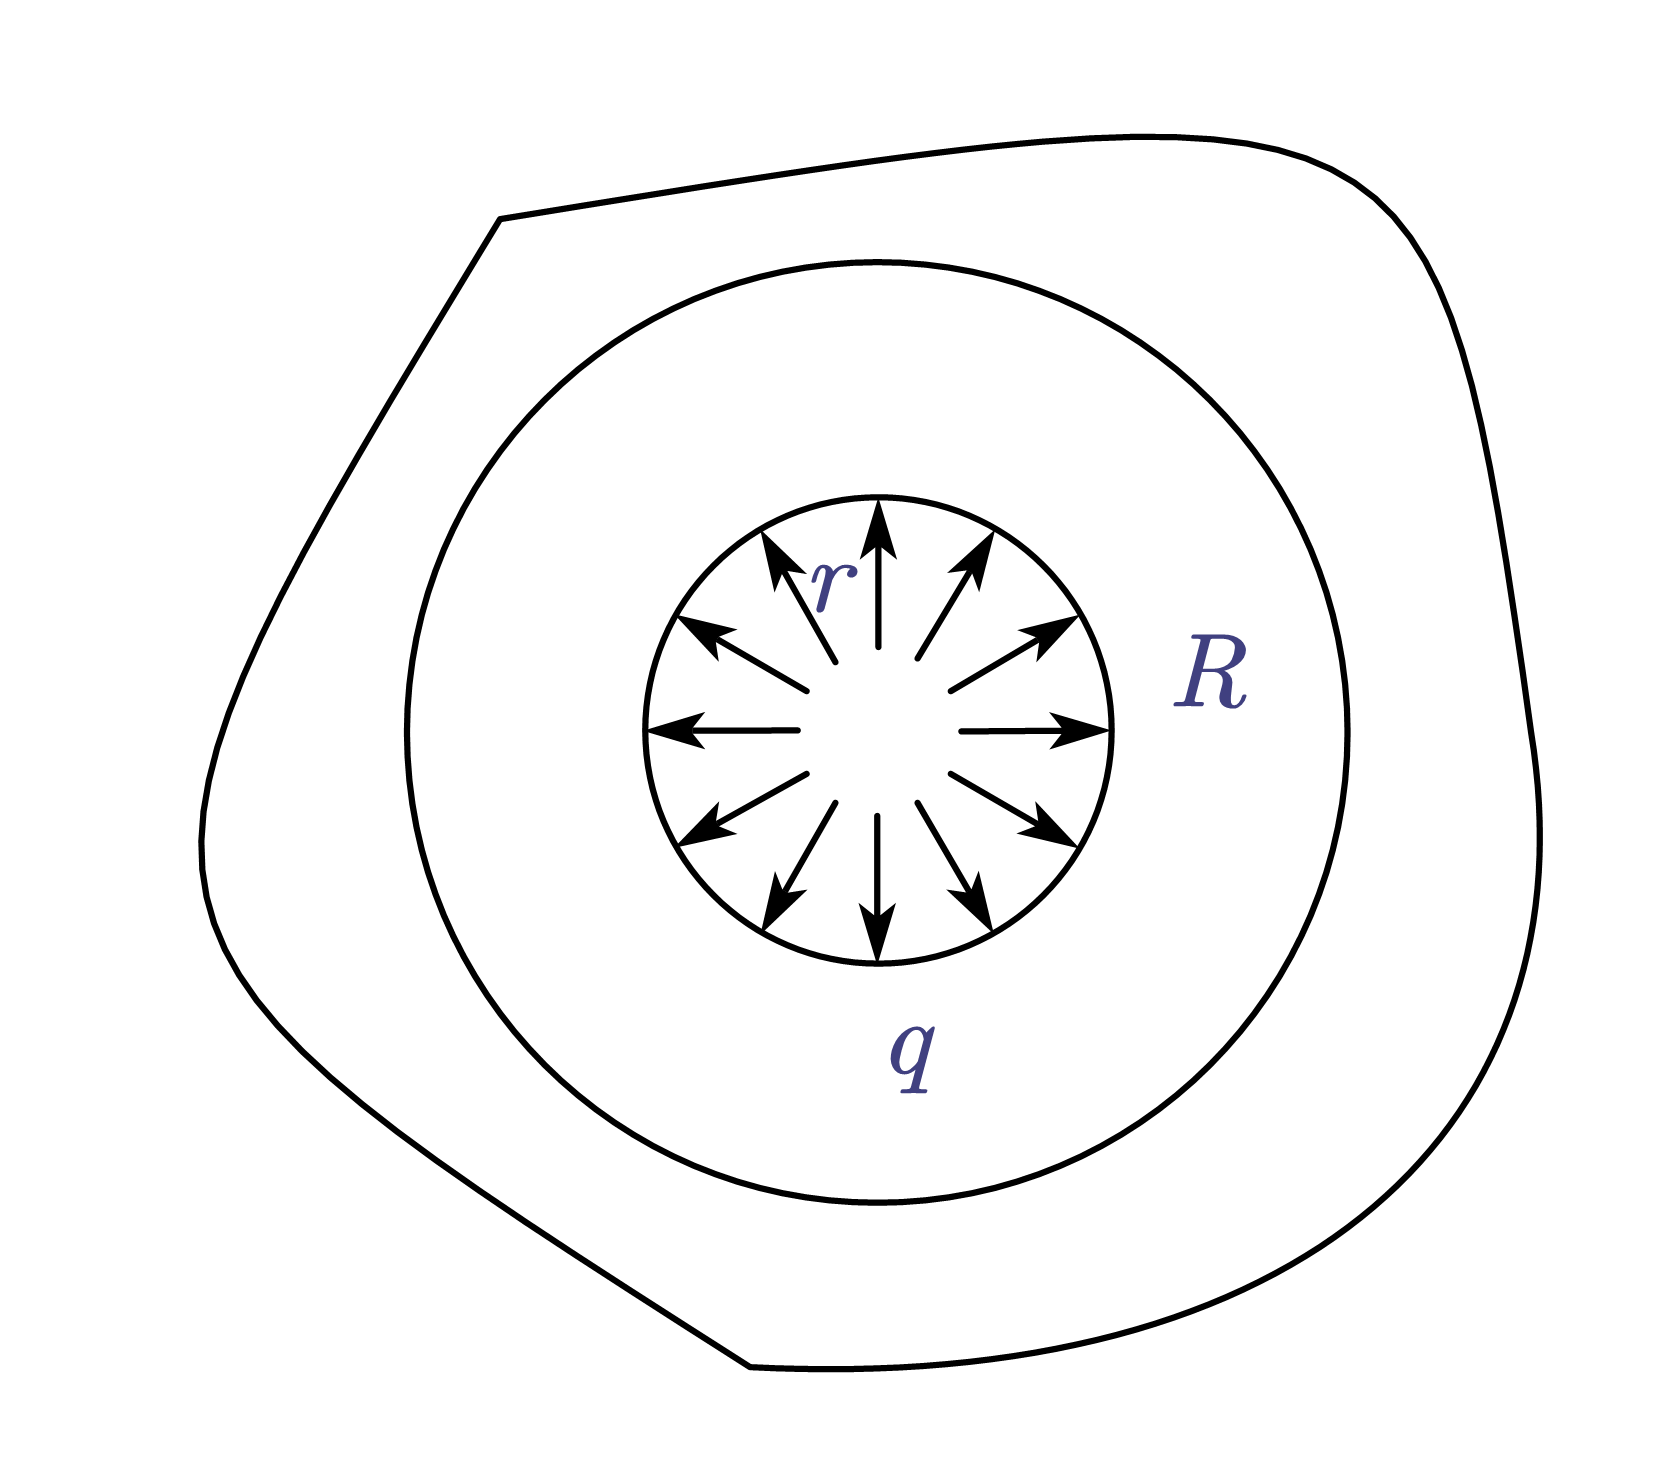
\includegraphics[scale=0.5]{figure/4-8.png}
\end{figure*}
	\begin{remark}
		圆筒轴对称应变问题的通解为:
		\[\begin{cases}
		\sigma _{\rho}=\frac{A}{\rho ^2}+2C\\
		\sigma _{\varphi}=-\frac{A}{\rho ^2}+2C\\
		\tau _{\rho \varphi}=0\\
		\end{cases}\]
		位移通解:\[\begin{cases}
		u_{\rho}=\frac{1+\mu}{E}\left[ -\frac{A}{\rho}+2\left( 1-2\mu \right) C\rho \right] +I\cos \varphi +K\sin \varphi\\
		u_{\varphi}=H\rho -I\sin \varphi +K\cos \varphi\\
		\end{cases}\]
		应力边界条件:\[\left( \sigma _{\rho} \right) _{\rho =r}=-q\]
		刚体是不可形变的,它能起到限制圆筒外边界径向位移的作用,因此位移边界条件:\[\left( u_{\rho} \right) _{\rho =R}=0\]
		解得:\[\begin{cases}
		A=\frac{-q}{\frac{1}{r^2}+\frac{1}{1-2\mu}\frac{1}{R^2}}\\
		C=\frac{-q}{2R^2\left( \frac{1-2\mu}{r^2}+\frac{1}{R^2} \right)}\\
		\end{cases}\Longrightarrow \begin{cases}
		\sigma _{\rho}=\frac{\frac{1-2\mu}{\rho ^2}+\frac{1}{R^2}}{\frac{1-2\mu}{r^2}+\frac{1}{R^2}}q\\
		\sigma _{\varphi}=\frac{\frac{1-2\mu}{\rho ^2}-\frac{1}{R^2}}{\frac{1-2\mu}{r^2}+\frac{1}{R^2}}q\\
		\end{cases}\]
	\end{remark}
	\begin{note}
		本题不能按照压力隧洞的方式求解,因为在外部与圆筒相接触的是一个刚体,而刚体是不能引用弹性力学的解答
	\end{note}

\subsection{曲梁的纯弯曲}
\subsubsection{问题及其描述}
矩形截面曲梁:内半径为$a$,外半径为$b$,在两端受有大小相等而转向相反的力偶$M$作用(梁的厚度为一个单位):$o$为曲梁的曲率转中心,两端面间极角为$\beta$,
\begin{figure}[H]
\centering
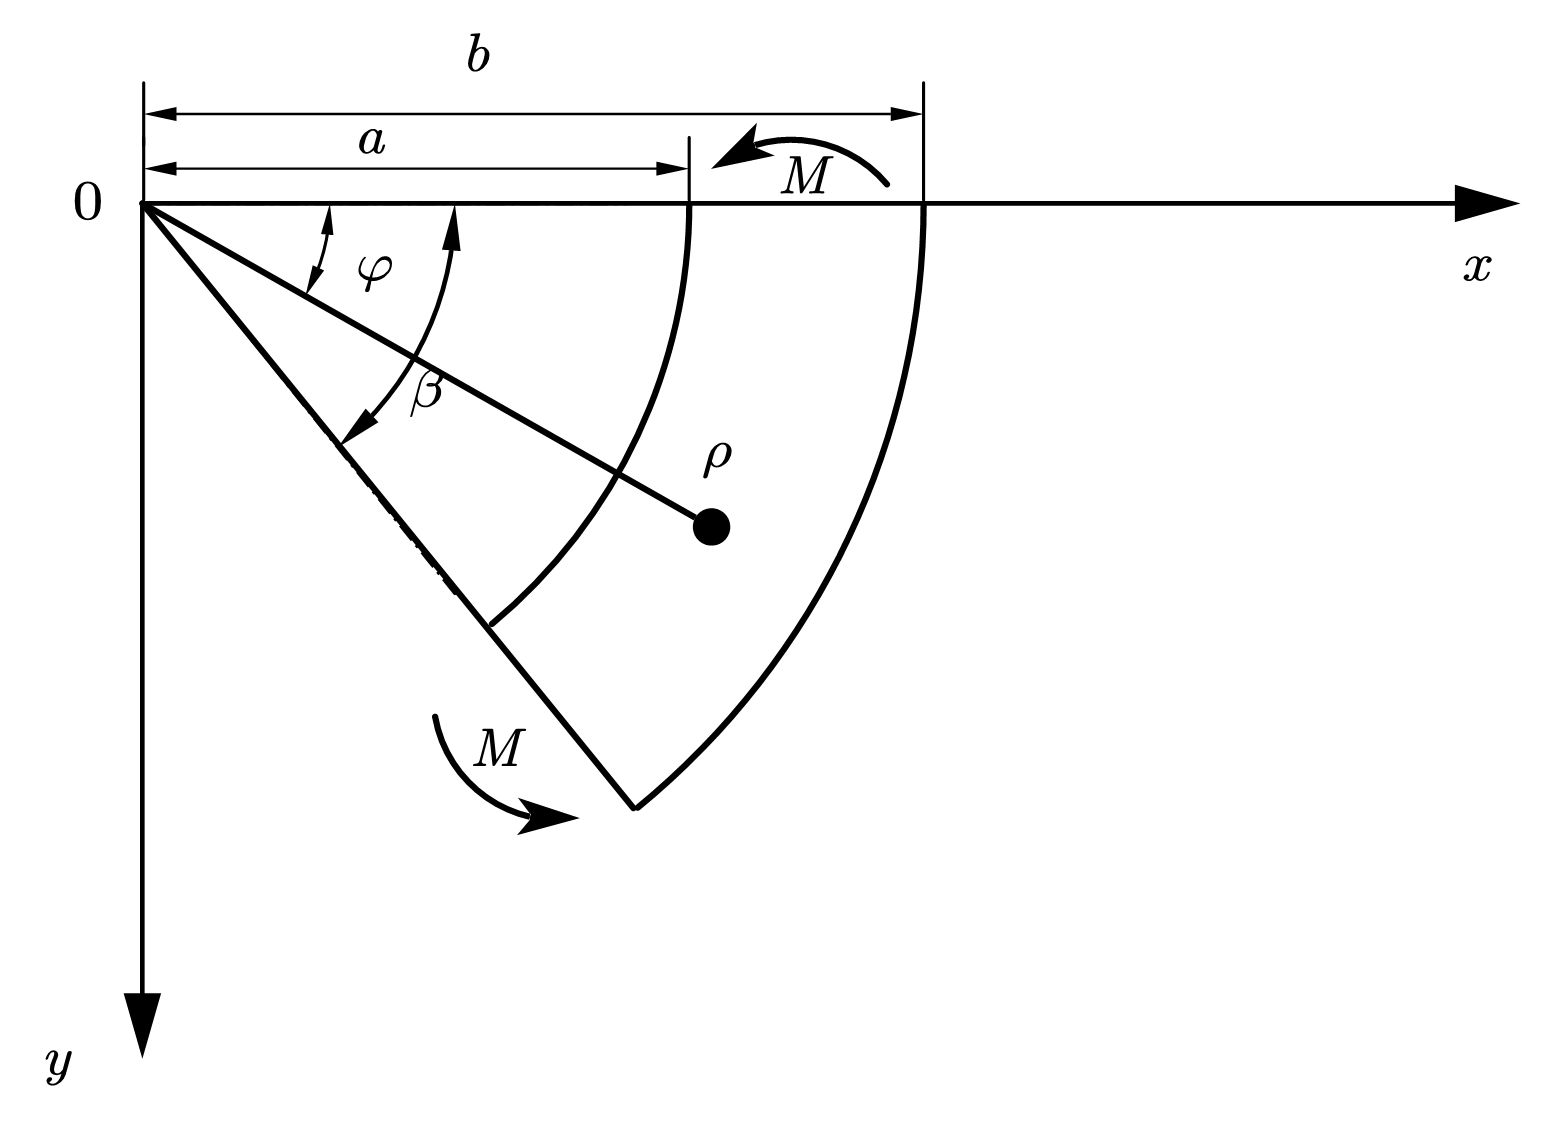
\includegraphics[scale=0.5]{figure/4-9.png}
\caption{}
\end{figure}
梁的全部边界都没有剪力。\\
在梁的内外两面,边界要求:$\left( \sigma _{\rho} \right) _{\rho =a}=0   ,   \left( \sigma _{\rho} \right) _{\rho =b}=0$\\
代入应力通解得:\[\begin{cases}
\frac{A}{a^2}+B\left( 1+\ln 2a \right) +2C=0\\
\frac{A}{b^2}+B\left( 1+\ln 2b \right) +2C=0\\
\end{cases}\]
根据圣维南原理,环向正应力$\sigma _{\varphi}$的主矢量应当为零,并合成弯矩$M$,因此要求:\[\int_a^b{\sigma _{\varphi}d\rho}=0   ,   \int_a^b{\rho \sigma _{\varphi}d\rho}=M\]
可求得:\[-\left( \varPhi \right) _{a}^{b}=M\]
即\[-\left( A\ln \frac{b}{a}+Bb^2\ln b+Cb^2+D \right) +\left( A\ln a+Ba^2\ln a+Ca^2+D \right) =-M\]
令$N=\left( \frac{b^2}{a^2}-1 \right) ^2-4\frac{b^2}{a^2}\left( \ln \frac{b}{a} \right) ^2$:
可得:\[\begin{cases}
A=\frac{4M}{N}\frac{b^2}{a^2}\ln \frac{b}{a}\\
B=\frac{2M}{a^2N}\left( \frac{b^2}{a^2}-1 \right)\\
C=-\frac{M}{a^2N}\left[ \frac{b^2}{a^2}-1+2\left( \frac{b^2}{a^2}\ln b-\ln a \right) \right]\\
\end{cases}\]
\begin{equation}
\begin{cases}
\sigma _{\rho}=-\frac{4M}{Na^2}\left( \frac{b^2}{a^2}\ln \frac{b}{\rho}+\ln \frac{\rho}{a}-\frac{b^2}{\rho ^2}\ln \frac{b}{a} \right)\\
\sigma _{\varphi}=\frac{4M}{Na^2}\left( \frac{b^2}{a^2}-1-\frac{b^2}{a^2}\ln \frac{b}{\rho}-\ln \frac{\rho}{a}-\frac{b^2}{\rho ^2}\ln \frac{b}{a} \right)\\
\tau _{\rho \varphi}=0\\
\end{cases}
\end{equation}
\begin{note}
	\quad
	\begin{enumerate}
		\item $\rho = a$,$\sigma _{\varphi}$取得最大值。
		\item 中性轴($\sigma _{\varphi}=0$距内侧纤维较近,离外侧较远,中心轴不在过截面形心。
		\item 与材料力学比较,$\sigma _{\varphi}$关于截面不再成双曲线分布,但曲率不大时这种情况影响较小,挤压应力$\sigma _{\rho}$实际不为零。
	\end{enumerate}
\end{note}
\begin{figure}[H]
	\centering
	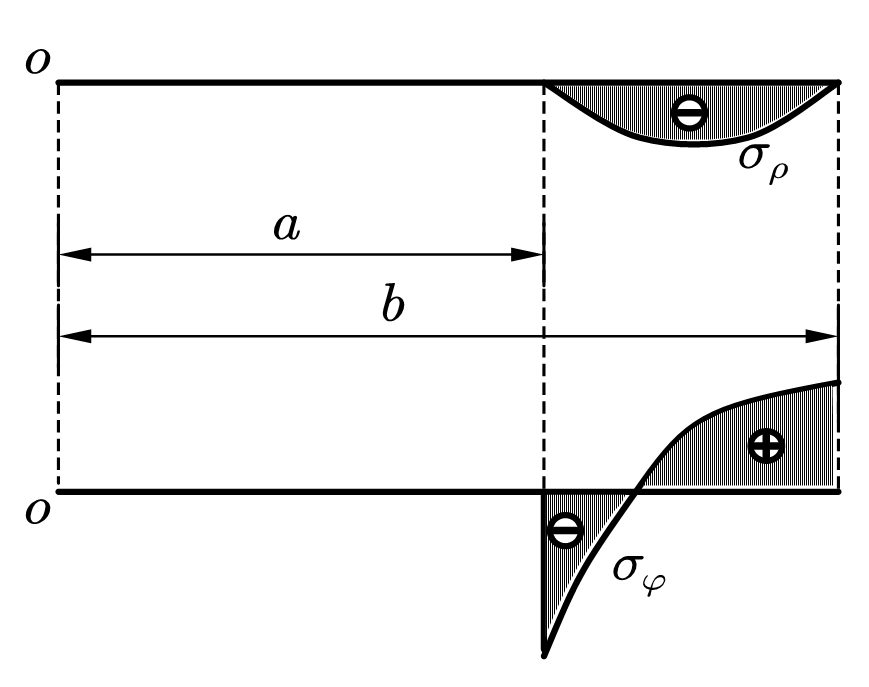
\includegraphics[scale=0.7]{figure/4-10.png}
	\caption{}
\end{figure}
\begin{example}
图示为带有一微小张角$\alpha$缺口的圆环,若将此圆环焊成一整环,试求此时圆环的内力矩$M$。
\begin{figure}[!h]
\centering
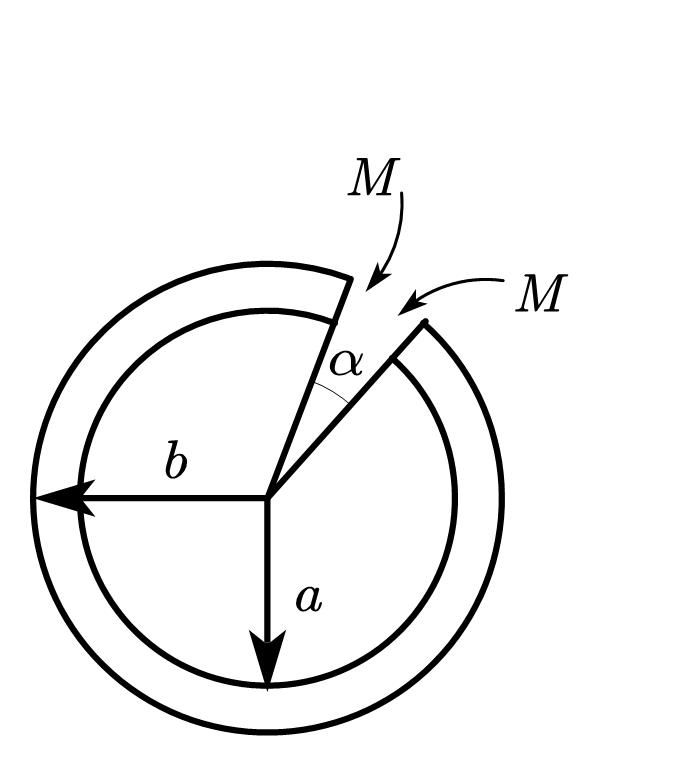
\includegraphics[scale=0.6]{figure/4-11.png}
\end{figure}
\end{example}
\begin{remark}
要使该圆环焊成一整环,需在两端加上一对平衡力矩$M$,使其产生环向位移$\delta =\rho \alpha $由两端受力偶作用时环向位移计算式\[u_{\varphi}=\frac{4B}{E}\rho \varphi +H\rho -I\sin \varphi +K\cos \varphi \]
可得:\[\left. u_{\varphi} \right|_{\varphi =2\pi}-\left. u_{\varphi} \right|_{\varphi =0}=\frac{8B\rho \pi}{E}=\delta =\rho \alpha \Rightarrow B=\frac{E\alpha}{8\pi}\]
代入$B$的计算式\[B=\frac{2M}{a^2N}\left( \frac{b^2}{a^2}-1 \right) \]
得:\[M=\frac{E\alpha a^4N}{16\pi \left( b^2-a^2 \right)}\]
\end{remark}

\subsection{圆孔的孔口应力集中}
背景:工程结构中常开设孔口,最简单的为圆孔,本节研究“小圆孔孔口应力集中问题”\\
小孔的条件:
\begin{enumerate}
\item 孔口尺寸$\ll $弹性体尺寸,孔口引起的应力扰动局限于小范围内。
\item 孔边距边界较远($>$1.5倍孔口尺寸),孔口与边界互不干扰。
\end{enumerate}
\begin{figure}[H]
	\centering
	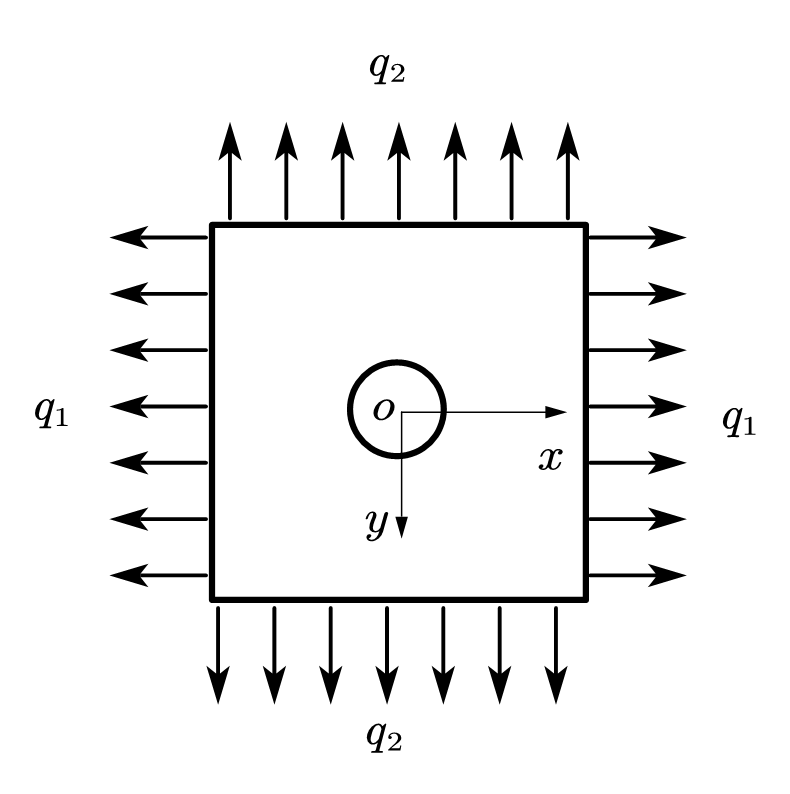
\includegraphics[scale=0.6]{figure/4-17.png}
\end{figure}
应力分量:\[\begin{cases}
\sigma _{\rho}=\frac{q_1+q_2}{2}\left( 1-\frac{a^2}{\rho ^2} \right) +\frac{q_1-q_2}{2}\left( 1-\frac{a^2}{\rho ^2} \right) \left( 1-3\frac{a^2}{\rho ^2} \right) \cos 2\varphi\\
\sigma _{\varphi}=\frac{q_1+q_2}{2}\left( 1+\frac{a^2}{\rho ^2} \right) -\frac{q_1-q_2}{2}\left( 1+3\frac{a^2}{\rho ^2} \right) \cos 2\varphi\\
\tau _{\varphi \rho}=-\frac{q_1-q_2}{2}\left( 1-\frac{a^2}{\rho ^2} \right) \left( 1+3\frac{a^2}{\rho ^2} \right) \sin 2\varphi\\
\end{cases}\]
\begin{example}
	在薄板距边界较远的某一点处,应力分量为$\sigma _x=\sigma _y=0,\tau _{xy}=q$如该处有一小圆孔,试求孔边的最大正应力。
\end{example}
\centerline{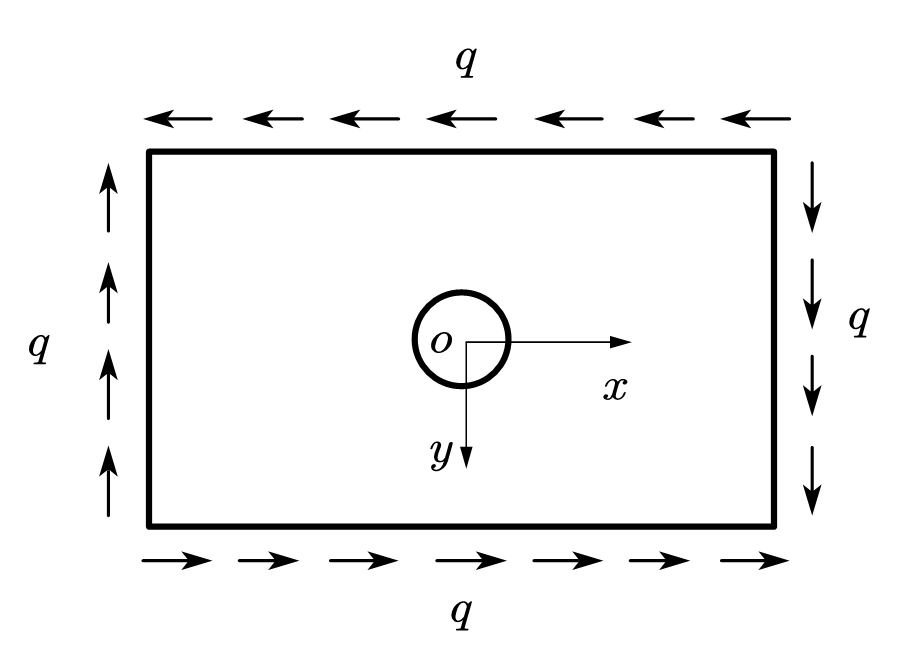
\includegraphics[scale=0.45]{figure/4-12.png}}
\begin{remark}
%	\begin{figure*}[!h]
%		\centering
%		\begin{minipage}[c]{0.35\textwidth}
%			\centering
%			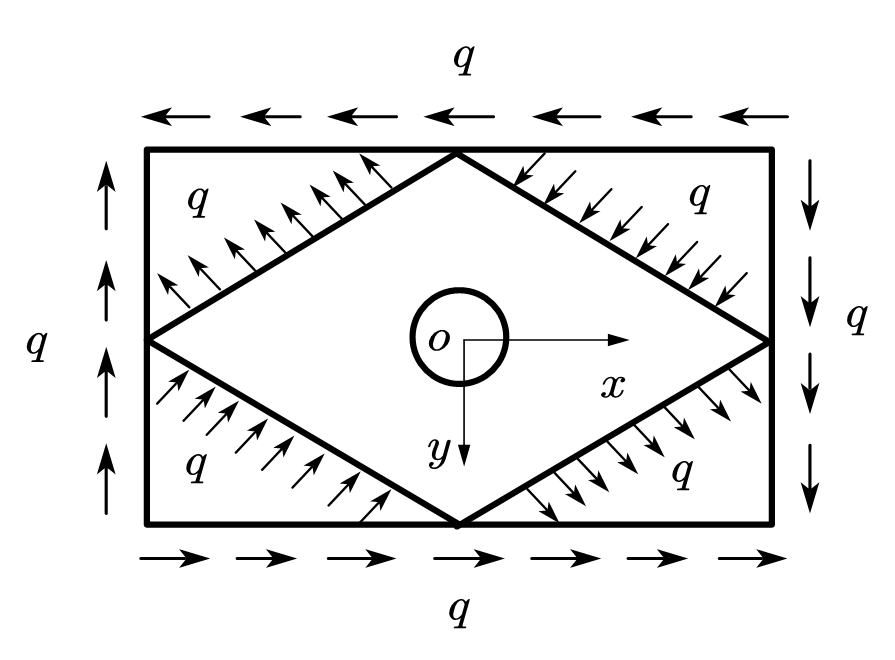
\includegraphics[scale=0.5]{figure/4-13.png}
%		\end{minipage}
%		\begin{minipage}[c]{0.35\textwidth}
%			\centering
%			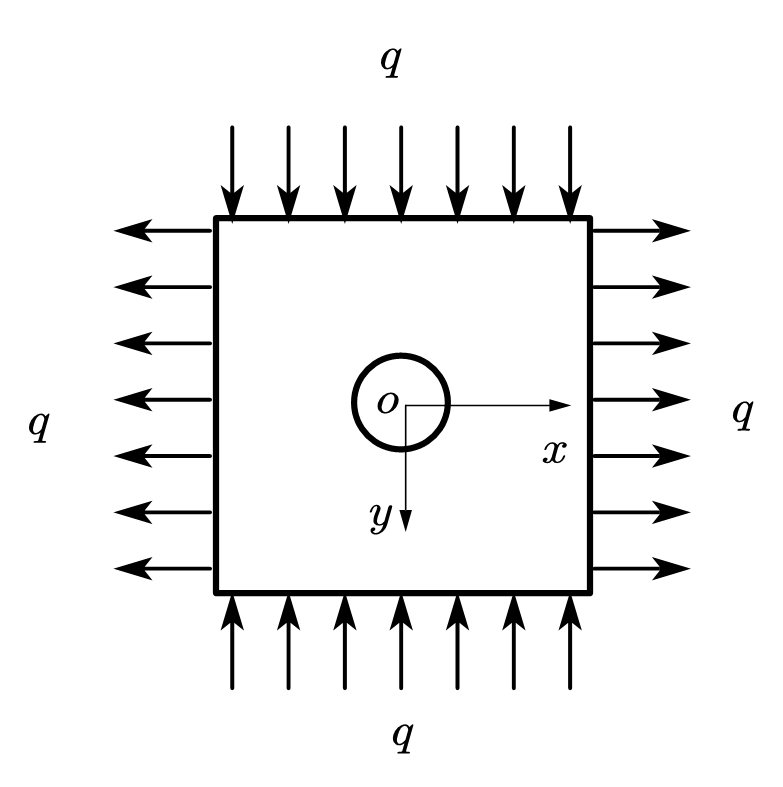
\includegraphics[scale=0.5]{figure/4-14.png}
%		\end{minipage}
%	\end{figure*}
经过等效转换可将问题转化为下问题\\
\centerline{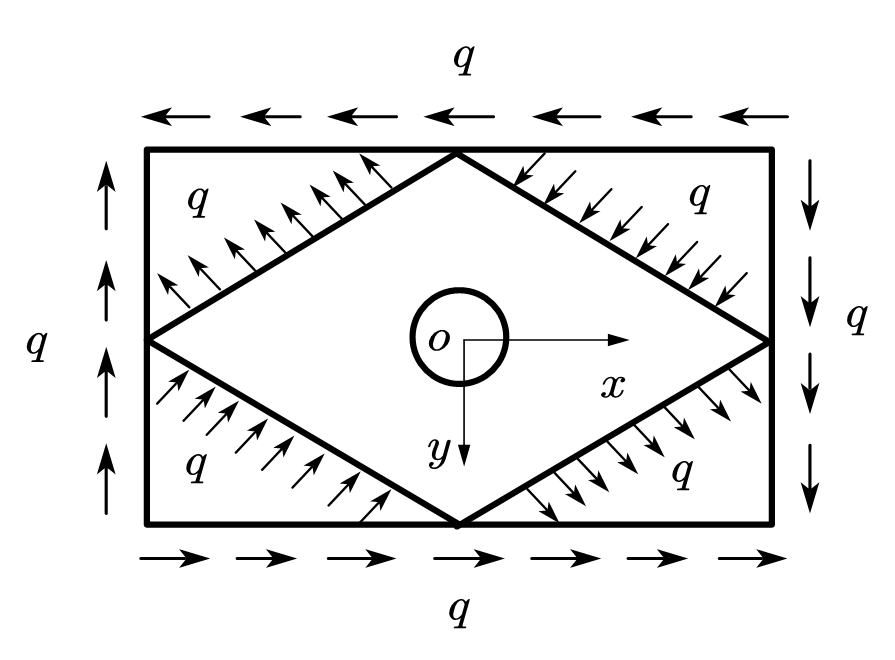
\includegraphics[scale=0.45]{figure/4-13.png}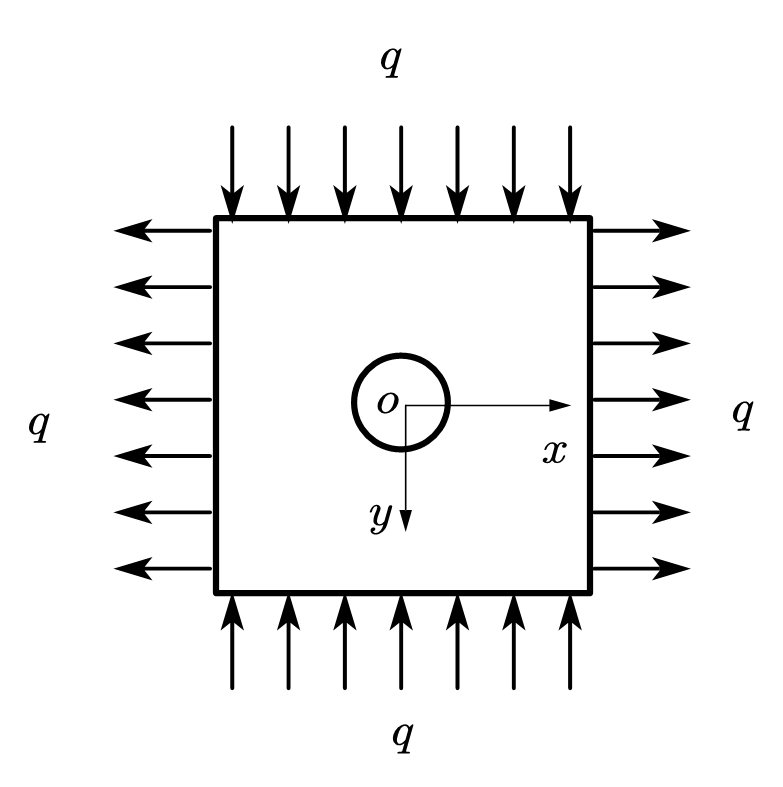
\includegraphics[scale=0.45]{figure/4-14.png}}\\
则\[\begin{cases}
\sigma _{\rho}=-q\left( 1-\frac{a^2}{\rho ^2} \right) \left( 1-3\frac{a^2}{\rho ^2} \right) \cos 2\varphi\\
\sigma _{\varphi}=-q\left( 1+3\frac{a^4}{\rho ^4} \right) \cos 2\varphi\\
\tau _{\rho \varphi}=-a\left( 1-\frac{a^2}{\rho ^2} \right) \left( 1+3\frac{a^2}{\rho ^2} \right) \sin 2\varphi\\
\end{cases}\]
将$\rho =a$代入得\[\begin{cases}
\sigma _{\rho}=0\\
\sigma _{\varphi}=-4q\cos 2\varphi\\
\tau _{\rho \varphi}=0\\
\end{cases}\]
则孔边最大应力为\[\begin{cases}
\sigma _{\rho}=0\\
\sigma _{\varphi}=\pm 4q\\
\tau _{\rho \varphi}=0\\
\end{cases}\]
\end{remark}

\subsection{楔形体问题-受集中力$F$作用}
\begin{example}
	如图所示,半无限平面体在边界上受有两条等值反向间距为$d$的等中力作用,单位宽度上集中力的值为$F$,设间距距$d$很小,试求其应力分量。
\end{example}
\centerline{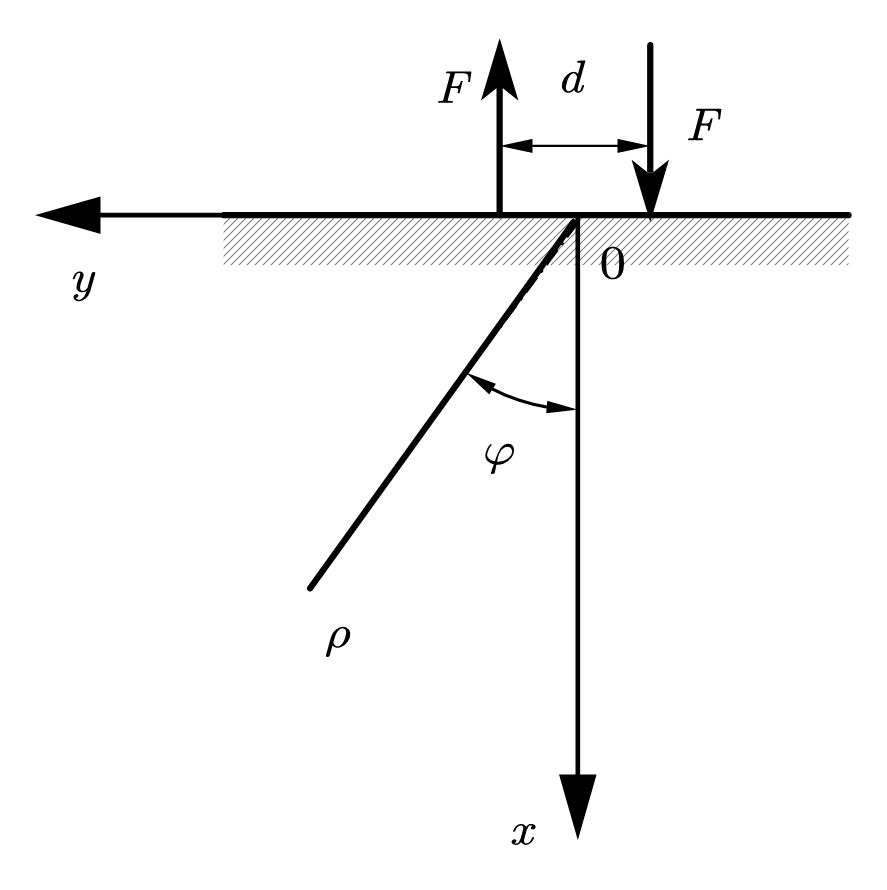
\includegraphics[scale=0.45]{figure/4-15.png}}
\begin{remark}
	原问题可以转化为\\
\centerline{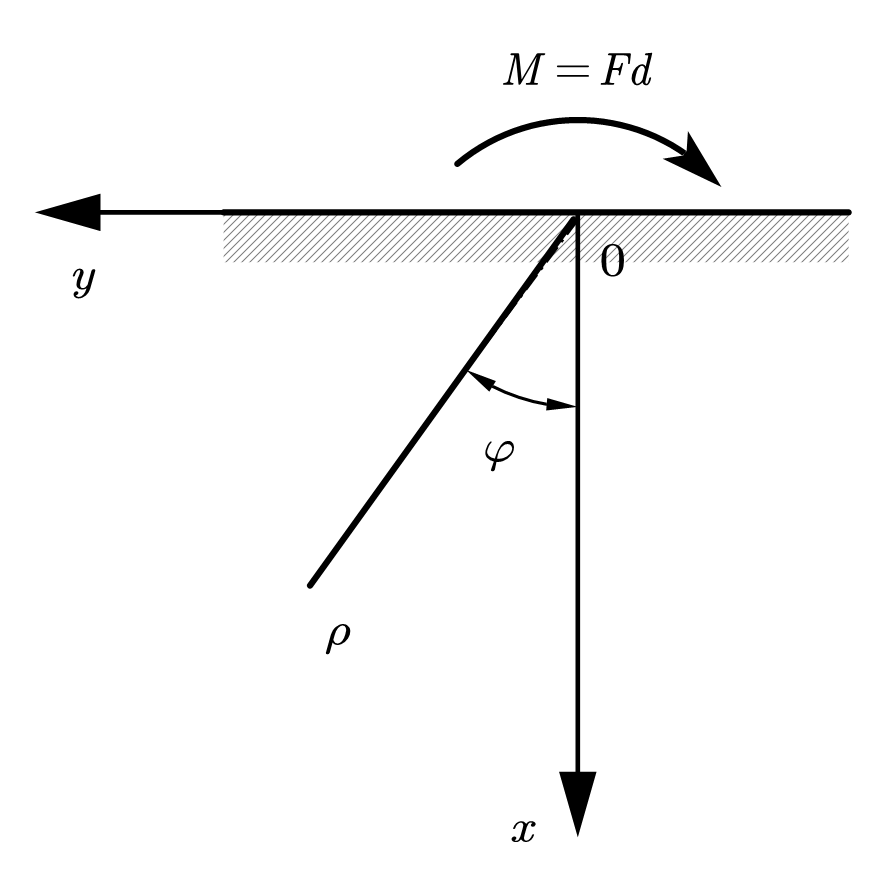
\includegraphics[scale=0.45]{figure/4-16.png}}
\[\begin{cases}
\sigma _{\rho}=\frac{2M\sin 2\varphi}{\left( \sin \alpha -\alpha \cos \alpha \right) \rho ^2}\\
\sigma _{\varphi}=0\\
\tau _{\rho \varphi}=-\frac{M\left( \cos 2\varphi -\cos \alpha \right)}{\left( \sin 2\alpha -\alpha \cos \alpha \right) \rho ^2}\\
\end{cases}\]
$\alpha =\pi $代入:\[\begin{cases}
\sigma _{\rho}=\frac{2M\sin 2\varphi}{\pi \rho ^2}\\
\sigma _{\varphi}=0\\
\tau _{\rho \varphi}=-\frac{M\left( \cos 2\varphi +1 \right)}{\pi \rho ^2}\\
\end{cases}\]
\end{remark}